% Capitolul 8: Estimatori de volatilitate
% Statistica piețelor financiare -- Program de licență, Academia de Studii Economice din București
% GENERAT de latex/build_chapter8.py -- modificați generatorul, nu acest fișier.

\newcommand{\coursename}{Statistica piețelor financiare}
\def\sfmlang{ro}
% Preambul comun SFM -- Statistica piețelor financiare / Statistics of Financial Markets (Beamer, 16:9)
% Același design ca MFM. Înainte de % Preambul comun SFM -- Statistica piețelor financiare / Statistics of Financial Markets (Beamer, 16:9)
% Același design ca MFM. Înainte de % Preambul comun SFM -- Statistica piețelor financiare / Statistics of Financial Markets (Beamer, 16:9)
% Același design ca MFM. Înainte de \input{../../latex/preamble} se definește
%   \newcommand{\coursename}{Statistics of Financial Markets}      (EN)
%   \newcommand{\coursename}{Statistica piețelor financiare}       (RO)  și  \def\sfmlang{ro}
% Fișierele .tex se află în EN/Courses, EN/Seminars, RO/Cursuri, RO/Seminarii (două niveluri sub rădăcină).
% Deck-urile sînt generate de latex/build_chapterN.py / build_seminarN.py (vezi latex/sfm_build.py).

\documentclass[9pt, aspectratio=169, t]{beamer}
\providecommand{\coursename}{Statistics of Financial Markets}

% Ensure content fits on slides
\setbeamersize{text margin left=8mm, text margin right=8mm}

%=============================================================================
% THEME AND STYLE CONFIGURATION
%=============================================================================
\usetheme{default}
% Using default theme for clean header/footer control

% Color Palette (matching Redispatch PDF)
\definecolor{MainBlue}{RGB}{26, 58, 110}
\definecolor{AccentBlue}{RGB}{26, 58, 110}
\definecolor{IDAred}{RGB}{205, 0, 0}
\definecolor{DarkGray}{RGB}{51, 51, 51}
\definecolor{MediumGray}{RGB}{128, 128, 128}
\definecolor{LightGray}{RGB}{248, 248, 248}
\definecolor{VeryLightGray}{RGB}{235, 235, 235}
\definecolor{KeynoteGray}{RGB}{218, 218, 218}
\definecolor{SectionGray}{RGB}{120, 120, 120}
\definecolor{FooterGray}{RGB}{100, 100, 100}
\definecolor{Crimson}{RGB}{220, 53, 69}
\definecolor{Forest}{RGB}{46, 125, 50}
\definecolor{Amber}{RGB}{181, 133, 63}
\definecolor{Orange}{RGB}{230, 126, 34}
\definecolor{Purple}{RGB}{142, 68, 173}

% Gradient background (exact Keynote 315° gradient: white to RGB 218,218,218)
\setbeamertemplate{background}{%
    \begin{tikzpicture}[remember picture, overlay]
        \shade[shading=axis, shading angle=315,
        top color=white, bottom color=KeynoteGray]
        (current page.south west) rectangle (current page.north east);
    \end{tikzpicture}%
}
% Fallback solid color for compatibility
\setbeamercolor{background canvas}{bg=}

\setbeamercolor{palette primary}{bg=MainBlue, fg=white}
\setbeamercolor{palette secondary}{bg=MainBlue!85, fg=white}
\setbeamercolor{palette tertiary}{bg=MainBlue!70, fg=white}
\setbeamercolor{structure}{fg=MainBlue}
\setbeamercolor{title}{fg=IDAred}
\setbeamercolor{frametitle}{fg=IDAred, bg=}
\setbeamercolor{block title}{bg=MainBlue, fg=white}
\setbeamercolor{block body}{bg=VeryLightGray, fg=DarkGray}
\setbeamercolor{block title alerted}{bg=Crimson, fg=white}
\setbeamercolor{block body alerted}{bg=Crimson!8, fg=DarkGray}
\setbeamercolor{block title example}{bg=Forest, fg=white}
\setbeamercolor{block body example}{bg=Forest!8, fg=DarkGray}
\setbeamercolor{item}{fg=MainBlue}

% Footer colors (override Madrid theme blue)
\setbeamercolor{author in head/foot}{fg=FooterGray, bg=}
\setbeamercolor{title in head/foot}{fg=FooterGray, bg=}
\setbeamercolor{date in head/foot}{fg=FooterGray, bg=}
\setbeamercolor{section in head/foot}{fg=FooterGray, bg=}
\setbeamercolor{subsection in head/foot}{fg=FooterGray, bg=}

% Bullet styles (apply everywhere including blocks)
\setbeamertemplate{itemize item}{\color{MainBlue}$\boxdot$}
\setbeamertemplate{itemize subitem}{\color{MainBlue}$\blacktriangleright$}
\setbeamertemplate{itemize subsubitem}{\color{MainBlue}\tiny$\bullet$}
\setbeamertemplate{itemize/enumerate body begin}{\normalsize}
\setbeamertemplate{itemize/enumerate subbody begin}{\normalsize}

% Item spacing - compact style
\setlength{\leftmargini}{10pt}       % Level 1: minimal indent
\setlength{\leftmarginii}{10pt}      % Level 2: minimal additional indent
% Compact list spacing (zero extra space before/after lists in blocks)
\makeatletter
\def\@listi{\leftmargin\leftmargini \topsep 0pt \parsep 0pt \itemsep 0pt}
\def\@listii{\leftmargin\leftmarginii \topsep 0pt \parsep 0pt \itemsep 0pt}
\makeatother

\setbeamertemplate{navigation symbols}{}

%=============================================================================
% CUSTOM HEADLINE
%=============================================================================
\setbeamertemplate{headline}{%
    \vskip10pt%
    \hbox to \paperwidth{%
        \hskip0.5cm%
        {\small\color{FooterGray}\renewcommand{\hyperlink}[2]{##2}\insertsectionhead}%
        \hfill%
        \textcolor{FooterGray}{\small\insertframenumber}%
        \hskip0.5cm%
    }%
    \vskip4pt%
    {\color{FooterGray}\hrule height 0.4pt}%
}

%=============================================================================
% CUSTOM FOOTER
%=============================================================================
\usepackage{fontawesome5}

\setbeamertemplate{footline}{%
    {\color{FooterGray}\hrule height 0.4pt}%
    \vskip4pt%
    \hbox to \paperwidth{%
        \hskip0.5cm%
        \textcolor{FooterGray}{\small\coursename}%
        \hfill%
        \raisebox{-0.1em}{%
            \begin{tikzpicture}[x=0.08em, y=0.08em, line width=0.4pt]
                \draw[FooterGray] (0,3) -- (1,4) -- (2,3.5) -- (3,5) -- (4,4) -- (5,6) -- (6,5.5) -- (7,4) -- (8,5) -- (9,7) -- (10,6) -- (11,5) -- (12,6.5) -- (13,8) -- (14,7) -- (15,6) -- (16,7.5) -- (17,9) -- (18,8) -- (19,7) -- (20,8.5) -- (21,10) -- (22,9) -- (23,8) -- (24,9.5);
            \end{tikzpicture}%
        }%
        \hskip0.5cm%
    }%
    \vskip6pt%
}

%=============================================================================
% PACKAGES
%=============================================================================
\usepackage[utf8]{inputenc}
\DeclareUnicodeCharacter{03B1}{\ensuremath{\alpha}}
\usepackage[T1]{fontenc}
\usepackage{amsmath, amssymb, amsthm}
\usepackage{mathtools}
\usepackage{bm}
\usepackage{tikz}
\usetikzlibrary{arrows.meta, positioning, shapes, calc, decorations.pathreplacing, shadings}
\usepackage{booktabs}
\usepackage{multirow}
\usepackage{array}
\usepackage{graphicx}
\usepackage{hyperref}
\usepackage{colortbl}
\usepackage{listings}
\lstset{language=Python, basicstyle=\ttfamily\scriptsize, keywordstyle=\color{MainBlue}\bfseries,
  commentstyle=\color{Forest}, stringstyle=\color{Crimson}, breaklines=true,
  frame=none, backgroundcolor=\color{VeryLightGray}, xleftmargin=2mm}
\hypersetup{colorlinks=true, linkcolor=MainBlue, urlcolor=MainBlue}
\graphicspath{{../../logos/}{../../charts/}{../../photos/}}
\usepackage{xcolor}
\hfuzz=2pt  % Suppress tiny overfull warnings (<2pt)
\vfuzz=2pt  % Suppress tiny vertical overfull warnings (<2pt)

%=============================================================================
% QUANTLET COMMANDS
%   \quantlet{<displayed name>}{<url>}       (generic, compatible with the older SFM decks)
%   \sfmquantlet{Ch_05}{SFM_ch5_garch}       -> https://github.com/danpele/SFM/tree/main/Quantlets/Ch_05/SFM_ch5_garch
%   \qlurl{<folder>} is defined per chapter by the generator (Quantlets/Ch_NN/<folder>)
%=============================================================================
\newcommand{\sfmrepo}{https://github.com/danpele/SFM}
\newcommand{\sfmqlbase}{https://github.com/danpele/SFM/tree/main/Quantlets}
\newcommand{\quantlet}[2]{%
    \hfill\href{#2}{%
        \raisebox{-0.15em}{
\includegraphics[height=0.7em]{ql_logo.png}}%
        \textcolor{MainBlue}{\tiny\ #1}%
    }%
}
\newcommand{\sfmquantlet}[2]{\quantlet{\detokenize{#2}}{\sfmqlbase/#1/#2}}

%=============================================================================
% NOTEBOOKS (Google Colab)
%   \colaburl{notebooks/EN/chapter5_seminar_notebook.ipynb} -> the Colab link of a file in the SFM repo
%   \nb: the chapter notebook (each seminar deck redefines it with \renewcommand)
%=============================================================================
\newcommand{\colaburl}[1]{https://colab.research.google.com/github/danpele/SFM/blob/main/#1}
\newcommand{\nb}{https://colab.research.google.com/github/danpele/SFM/tree/main/notebooks/EN}
\newcommand{\nbname}{notebooks/EN}

%=============================================================================
% SLIDE HELPERS (used by the generators; the same as in MFM)
%=============================================================================
% local font size for list bodies (the preamble forces \normalsize)
\newcommand{\itemsize}[1]{\setbeamertemplate{itemize/enumerate body begin}{#1}\setbeamertemplate{itemize/enumerate subbody begin}{#1}}
\newcommand{\intitle}[1]{{\hypersetup{urlcolor=white}#1}}   % white links inside coloured title bars
\newcommand{\imgcap}[1]{{\scriptsize #1}\\[0.5mm]}          % caption under a photo
\newcommand{\imgcredit}[2]{{\tiny\color{FooterGray}\href{#1}{#2}}}   % image credit: source URL, author/licence
\newcommand{\aiprompt}[1]{{\ttfamily\color{MainBlue}#1}}     % a prompt to an AI assistant

%=============================================================================
% SEMINARS: student version by default; the instructor wrapper *_solutions.tex sets \solutionstrue
%=============================================================================
\makeatletter\@ifundefined{ifsolutions}{\expandafter\newif\csname ifsolutions\endcsname}{}\makeatother
\newcommand{\solonly}[1]{\ifsolutions #1\fi}
\newcommand{\propsub}{\ifsolutions\else\framesubtitle{\ifdefined\sfmlang Rezolvarea se discută la seminar\else Solution discussed in class\fi}\fi}

%=============================================================================
% APPENDIX AND CHAPTER LINKS (latex/appendix_links.py writes the calls; it also re-declares these
% macros before \begin{document}, so the decks compile with or without this preamble block)
%=============================================================================
\providecommand{\sfmapplink}[3]{\hypertarget{#2}{}\hyperlink{#1}{\beamergotobutton{#3}}}
\providecommand{\sfmappback}[2]{\begin{tikzpicture}[remember picture,overlay]\node[anchor=south east] at ([xshift=-3mm,yshift=7mm]current page.south east){\hyperlink{#1}{\beamerreturnbutton{#2}}};\end{tikzpicture}}
\providecommand{\sfmchlink}[2]{\href{#1}{#2}}
\providecommand{\sfmchlinkt}[2]{\href{#1}{\usebeamercolor[fg]{frametitle}#2}}

%=============================================================================
% QUANTINAR COMMAND: link către un curs Quantinar (subiecte avansate)
%=============================================================================
\newcommand{\quantinar}[2]{%
    \href{#2}{%
        \raisebox{-0.15em}{
\includegraphics[height=0.8em]{qr_logo.png}}%
        \textcolor{MainBlue}{\scriptsize\ #1}%
    }%
}

%=============================================================================
% CUSTOM TITLE PAGE
%=============================================================================
\defbeamertemplate*{title page}{hybrid}[1][]
{
    \vspace{0.2cm}
    % Logos row - top header (with clickable links)
    \begin{center}
        \href{https://www.ase.ro}{
\includegraphics[height=1.0cm]{ase_logo.png}}\hspace{0.3cm}%
        \href{https://theida.net}{
\includegraphics[height=1.0cm]{ida_logo.png}}\hspace{0.3cm}%
        \href{https://blockchain-research-center.com}{
\includegraphics[height=1.0cm]{brc_logo.png}}\hspace{0.3cm}%
        \href{https://www.ai4efin.ase.ro}{
\includegraphics[height=1.0cm]{ai4efin_logo.png}}\hspace{0.3cm}%
        \href{https://ipe.ro/new}{
\includegraphics[height=1.0cm]{acad_logo.png}}\hspace{0.3cm}%
        \href{https://www.digital-finance-msca.com}{
\includegraphics[height=1.0cm]{msca_logo.png}}%
    \end{center}

    \vspace{0.6cm}

    % Main title with Q logos on sides (with clickable links)
    \begin{center}
        \begin{minipage}{0.1\textwidth}
            \centering
            \href{https://quantlet.com}{
\includegraphics[height=1.1cm]{ql_logo.png}}
        \end{minipage}%
        \begin{minipage}{0.78\textwidth}
            \centering
            {\LARGE\bfseries\usebeamercolor[fg]{title}\inserttitle}

            \vspace{0.3cm}

            {\usebeamerfont{subtitle}\usebeamercolor[fg]{title}\insertsubtitle}
        \end{minipage}%
        \begin{minipage}{0.1\textwidth}
            \centering
            \href{https://quantinar.com}{
\includegraphics[height=1.1cm]{qr_logo.png}}
        \end{minipage}
    \end{center}

    \vspace{0.6cm}

    % Authors (left aligned)
    \hspace{0.5cm}{\usebeamerfont{author}\insertauthor}

    \vspace{0.3cm}

    % Institute/Affiliations (left aligned)
    \hspace{0.5cm}\begin{minipage}[t]{0.9\textwidth}
        \raggedright\small\insertinstitute
    \end{minipage}
}

%=============================================================================
% THEOREM ENVIRONMENTS
%=============================================================================
\theoremstyle{definition}
\setbeamertemplate{theorems}[numbered]
\ifdefined\sfmlang
\newtheorem{defn}{Definiție}
\newtheorem{thm}{Teoremă}
\newtheorem{prop}{Propoziție}
\newtheorem{rmk}{Observație}
\else
\newtheorem{defn}{Definition}
\newtheorem{thm}{Theorem}
\newtheorem{prop}{Proposition}
\newtheorem{rmk}{Remark}
\fi

%=============================================================================
% CENTRED MINIPAGE (no extra vertical space)
%=============================================================================
\newenvironment{cminipage}[1]{%
    \par\noindent\hfill\begin{minipage}{#1}\ignorespaces
}{%
    \end{minipage}\hfill\null\par
}

%=============================================================================
% CUSTOM COMMANDS
%=============================================================================
\newcommand{\E}{\mathbb{E}}
\newcommand{\Var}{\text{Var}}
\newcommand{\Cov}{\text{Cov}}
\newcommand{\Corr}{\text{Corr}}
\newcommand{\R}{\mathbb{R}}
\newcommand{\N}{\mathbb{N}}
\newcommand{\Z}{\mathbb{Z}}
\newcommand{\B}{\mathbf{B}}
\newcommand{\imark}{\textcolor{MainBlue}{\textbullet}}
\newcommand{\RMSE}{\text{RMSE}}
\newcommand{\MAE}{\text{MAE}}
\newcommand{\MAPE}{\text{MAPE}}

 se definește
%   \newcommand{\coursename}{Statistics of Financial Markets}      (EN)
%   \newcommand{\coursename}{Statistica piețelor financiare}       (RO)  și  \def\sfmlang{ro}
% Fișierele .tex se află în EN/Courses, EN/Seminars, RO/Cursuri, RO/Seminarii (două niveluri sub rădăcină).
% Deck-urile sînt generate de latex/build_chapterN.py / build_seminarN.py (vezi latex/sfm_build.py).

\documentclass[9pt, aspectratio=169, t]{beamer}
\providecommand{\coursename}{Statistics of Financial Markets}

% Ensure content fits on slides
\setbeamersize{text margin left=8mm, text margin right=8mm}

%=============================================================================
% THEME AND STYLE CONFIGURATION
%=============================================================================
\usetheme{default}
% Using default theme for clean header/footer control

% Color Palette (matching Redispatch PDF)
\definecolor{MainBlue}{RGB}{26, 58, 110}
\definecolor{AccentBlue}{RGB}{26, 58, 110}
\definecolor{IDAred}{RGB}{205, 0, 0}
\definecolor{DarkGray}{RGB}{51, 51, 51}
\definecolor{MediumGray}{RGB}{128, 128, 128}
\definecolor{LightGray}{RGB}{248, 248, 248}
\definecolor{VeryLightGray}{RGB}{235, 235, 235}
\definecolor{KeynoteGray}{RGB}{218, 218, 218}
\definecolor{SectionGray}{RGB}{120, 120, 120}
\definecolor{FooterGray}{RGB}{100, 100, 100}
\definecolor{Crimson}{RGB}{220, 53, 69}
\definecolor{Forest}{RGB}{46, 125, 50}
\definecolor{Amber}{RGB}{181, 133, 63}
\definecolor{Orange}{RGB}{230, 126, 34}
\definecolor{Purple}{RGB}{142, 68, 173}

% Gradient background (exact Keynote 315° gradient: white to RGB 218,218,218)
\setbeamertemplate{background}{%
    \begin{tikzpicture}[remember picture, overlay]
        \shade[shading=axis, shading angle=315,
        top color=white, bottom color=KeynoteGray]
        (current page.south west) rectangle (current page.north east);
    \end{tikzpicture}%
}
% Fallback solid color for compatibility
\setbeamercolor{background canvas}{bg=}

\setbeamercolor{palette primary}{bg=MainBlue, fg=white}
\setbeamercolor{palette secondary}{bg=MainBlue!85, fg=white}
\setbeamercolor{palette tertiary}{bg=MainBlue!70, fg=white}
\setbeamercolor{structure}{fg=MainBlue}
\setbeamercolor{title}{fg=IDAred}
\setbeamercolor{frametitle}{fg=IDAred, bg=}
\setbeamercolor{block title}{bg=MainBlue, fg=white}
\setbeamercolor{block body}{bg=VeryLightGray, fg=DarkGray}
\setbeamercolor{block title alerted}{bg=Crimson, fg=white}
\setbeamercolor{block body alerted}{bg=Crimson!8, fg=DarkGray}
\setbeamercolor{block title example}{bg=Forest, fg=white}
\setbeamercolor{block body example}{bg=Forest!8, fg=DarkGray}
\setbeamercolor{item}{fg=MainBlue}

% Footer colors (override Madrid theme blue)
\setbeamercolor{author in head/foot}{fg=FooterGray, bg=}
\setbeamercolor{title in head/foot}{fg=FooterGray, bg=}
\setbeamercolor{date in head/foot}{fg=FooterGray, bg=}
\setbeamercolor{section in head/foot}{fg=FooterGray, bg=}
\setbeamercolor{subsection in head/foot}{fg=FooterGray, bg=}

% Bullet styles (apply everywhere including blocks)
\setbeamertemplate{itemize item}{\color{MainBlue}$\boxdot$}
\setbeamertemplate{itemize subitem}{\color{MainBlue}$\blacktriangleright$}
\setbeamertemplate{itemize subsubitem}{\color{MainBlue}\tiny$\bullet$}
\setbeamertemplate{itemize/enumerate body begin}{\normalsize}
\setbeamertemplate{itemize/enumerate subbody begin}{\normalsize}

% Item spacing - compact style
\setlength{\leftmargini}{10pt}       % Level 1: minimal indent
\setlength{\leftmarginii}{10pt}      % Level 2: minimal additional indent
% Compact list spacing (zero extra space before/after lists in blocks)
\makeatletter
\def\@listi{\leftmargin\leftmargini \topsep 0pt \parsep 0pt \itemsep 0pt}
\def\@listii{\leftmargin\leftmarginii \topsep 0pt \parsep 0pt \itemsep 0pt}
\makeatother

\setbeamertemplate{navigation symbols}{}

%=============================================================================
% CUSTOM HEADLINE
%=============================================================================
\setbeamertemplate{headline}{%
    \vskip10pt%
    \hbox to \paperwidth{%
        \hskip0.5cm%
        {\small\color{FooterGray}\renewcommand{\hyperlink}[2]{##2}\insertsectionhead}%
        \hfill%
        \textcolor{FooterGray}{\small\insertframenumber}%
        \hskip0.5cm%
    }%
    \vskip4pt%
    {\color{FooterGray}\hrule height 0.4pt}%
}

%=============================================================================
% CUSTOM FOOTER
%=============================================================================
\usepackage{fontawesome5}

\setbeamertemplate{footline}{%
    {\color{FooterGray}\hrule height 0.4pt}%
    \vskip4pt%
    \hbox to \paperwidth{%
        \hskip0.5cm%
        \textcolor{FooterGray}{\small\coursename}%
        \hfill%
        \raisebox{-0.1em}{%
            \begin{tikzpicture}[x=0.08em, y=0.08em, line width=0.4pt]
                \draw[FooterGray] (0,3) -- (1,4) -- (2,3.5) -- (3,5) -- (4,4) -- (5,6) -- (6,5.5) -- (7,4) -- (8,5) -- (9,7) -- (10,6) -- (11,5) -- (12,6.5) -- (13,8) -- (14,7) -- (15,6) -- (16,7.5) -- (17,9) -- (18,8) -- (19,7) -- (20,8.5) -- (21,10) -- (22,9) -- (23,8) -- (24,9.5);
            \end{tikzpicture}%
        }%
        \hskip0.5cm%
    }%
    \vskip6pt%
}

%=============================================================================
% PACKAGES
%=============================================================================
\usepackage[utf8]{inputenc}
\DeclareUnicodeCharacter{03B1}{\ensuremath{\alpha}}
\usepackage[T1]{fontenc}
\usepackage{amsmath, amssymb, amsthm}
\usepackage{mathtools}
\usepackage{bm}
\usepackage{tikz}
\usetikzlibrary{arrows.meta, positioning, shapes, calc, decorations.pathreplacing, shadings}
\usepackage{booktabs}
\usepackage{multirow}
\usepackage{array}
\usepackage{graphicx}
\usepackage{hyperref}
\usepackage{colortbl}
\usepackage{listings}
\lstset{language=Python, basicstyle=\ttfamily\scriptsize, keywordstyle=\color{MainBlue}\bfseries,
  commentstyle=\color{Forest}, stringstyle=\color{Crimson}, breaklines=true,
  frame=none, backgroundcolor=\color{VeryLightGray}, xleftmargin=2mm}
\hypersetup{colorlinks=true, linkcolor=MainBlue, urlcolor=MainBlue}
\graphicspath{{../../logos/}{../../charts/}{../../photos/}}
\usepackage{xcolor}
\hfuzz=2pt  % Suppress tiny overfull warnings (<2pt)
\vfuzz=2pt  % Suppress tiny vertical overfull warnings (<2pt)

%=============================================================================
% QUANTLET COMMANDS
%   \quantlet{<displayed name>}{<url>}       (generic, compatible with the older SFM decks)
%   \sfmquantlet{Ch_05}{SFM_ch5_garch}       -> https://github.com/danpele/SFM/tree/main/Quantlets/Ch_05/SFM_ch5_garch
%   \qlurl{<folder>} is defined per chapter by the generator (Quantlets/Ch_NN/<folder>)
%=============================================================================
\newcommand{\sfmrepo}{https://github.com/danpele/SFM}
\newcommand{\sfmqlbase}{https://github.com/danpele/SFM/tree/main/Quantlets}
\newcommand{\quantlet}[2]{%
    \hfill\href{#2}{%
        \raisebox{-0.15em}{
\includegraphics[height=0.7em]{ql_logo.png}}%
        \textcolor{MainBlue}{\tiny\ #1}%
    }%
}
\newcommand{\sfmquantlet}[2]{\quantlet{\detokenize{#2}}{\sfmqlbase/#1/#2}}

%=============================================================================
% NOTEBOOKS (Google Colab)
%   \colaburl{notebooks/EN/chapter5_seminar_notebook.ipynb} -> the Colab link of a file in the SFM repo
%   \nb: the chapter notebook (each seminar deck redefines it with \renewcommand)
%=============================================================================
\newcommand{\colaburl}[1]{https://colab.research.google.com/github/danpele/SFM/blob/main/#1}
\newcommand{\nb}{https://colab.research.google.com/github/danpele/SFM/tree/main/notebooks/EN}
\newcommand{\nbname}{notebooks/EN}

%=============================================================================
% SLIDE HELPERS (used by the generators; the same as in MFM)
%=============================================================================
% local font size for list bodies (the preamble forces \normalsize)
\newcommand{\itemsize}[1]{\setbeamertemplate{itemize/enumerate body begin}{#1}\setbeamertemplate{itemize/enumerate subbody begin}{#1}}
\newcommand{\intitle}[1]{{\hypersetup{urlcolor=white}#1}}   % white links inside coloured title bars
\newcommand{\imgcap}[1]{{\scriptsize #1}\\[0.5mm]}          % caption under a photo
\newcommand{\imgcredit}[2]{{\tiny\color{FooterGray}\href{#1}{#2}}}   % image credit: source URL, author/licence
\newcommand{\aiprompt}[1]{{\ttfamily\color{MainBlue}#1}}     % a prompt to an AI assistant

%=============================================================================
% SEMINARS: student version by default; the instructor wrapper *_solutions.tex sets \solutionstrue
%=============================================================================
\makeatletter\@ifundefined{ifsolutions}{\expandafter\newif\csname ifsolutions\endcsname}{}\makeatother
\newcommand{\solonly}[1]{\ifsolutions #1\fi}
\newcommand{\propsub}{\ifsolutions\else\framesubtitle{\ifdefined\sfmlang Rezolvarea se discută la seminar\else Solution discussed in class\fi}\fi}

%=============================================================================
% APPENDIX AND CHAPTER LINKS (latex/appendix_links.py writes the calls; it also re-declares these
% macros before \begin{document}, so the decks compile with or without this preamble block)
%=============================================================================
\providecommand{\sfmapplink}[3]{\hypertarget{#2}{}\hyperlink{#1}{\beamergotobutton{#3}}}
\providecommand{\sfmappback}[2]{\begin{tikzpicture}[remember picture,overlay]\node[anchor=south east] at ([xshift=-3mm,yshift=7mm]current page.south east){\hyperlink{#1}{\beamerreturnbutton{#2}}};\end{tikzpicture}}
\providecommand{\sfmchlink}[2]{\href{#1}{#2}}
\providecommand{\sfmchlinkt}[2]{\href{#1}{\usebeamercolor[fg]{frametitle}#2}}

%=============================================================================
% QUANTINAR COMMAND: link către un curs Quantinar (subiecte avansate)
%=============================================================================
\newcommand{\quantinar}[2]{%
    \href{#2}{%
        \raisebox{-0.15em}{
\includegraphics[height=0.8em]{qr_logo.png}}%
        \textcolor{MainBlue}{\scriptsize\ #1}%
    }%
}

%=============================================================================
% CUSTOM TITLE PAGE
%=============================================================================
\defbeamertemplate*{title page}{hybrid}[1][]
{
    \vspace{0.2cm}
    % Logos row - top header (with clickable links)
    \begin{center}
        \href{https://www.ase.ro}{
\includegraphics[height=1.0cm]{ase_logo.png}}\hspace{0.3cm}%
        \href{https://theida.net}{
\includegraphics[height=1.0cm]{ida_logo.png}}\hspace{0.3cm}%
        \href{https://blockchain-research-center.com}{
\includegraphics[height=1.0cm]{brc_logo.png}}\hspace{0.3cm}%
        \href{https://www.ai4efin.ase.ro}{
\includegraphics[height=1.0cm]{ai4efin_logo.png}}\hspace{0.3cm}%
        \href{https://ipe.ro/new}{
\includegraphics[height=1.0cm]{acad_logo.png}}\hspace{0.3cm}%
        \href{https://www.digital-finance-msca.com}{
\includegraphics[height=1.0cm]{msca_logo.png}}%
    \end{center}

    \vspace{0.6cm}

    % Main title with Q logos on sides (with clickable links)
    \begin{center}
        \begin{minipage}{0.1\textwidth}
            \centering
            \href{https://quantlet.com}{
\includegraphics[height=1.1cm]{ql_logo.png}}
        \end{minipage}%
        \begin{minipage}{0.78\textwidth}
            \centering
            {\LARGE\bfseries\usebeamercolor[fg]{title}\inserttitle}

            \vspace{0.3cm}

            {\usebeamerfont{subtitle}\usebeamercolor[fg]{title}\insertsubtitle}
        \end{minipage}%
        \begin{minipage}{0.1\textwidth}
            \centering
            \href{https://quantinar.com}{
\includegraphics[height=1.1cm]{qr_logo.png}}
        \end{minipage}
    \end{center}

    \vspace{0.6cm}

    % Authors (left aligned)
    \hspace{0.5cm}{\usebeamerfont{author}\insertauthor}

    \vspace{0.3cm}

    % Institute/Affiliations (left aligned)
    \hspace{0.5cm}\begin{minipage}[t]{0.9\textwidth}
        \raggedright\small\insertinstitute
    \end{minipage}
}

%=============================================================================
% THEOREM ENVIRONMENTS
%=============================================================================
\theoremstyle{definition}
\setbeamertemplate{theorems}[numbered]
\ifdefined\sfmlang
\newtheorem{defn}{Definiție}
\newtheorem{thm}{Teoremă}
\newtheorem{prop}{Propoziție}
\newtheorem{rmk}{Observație}
\else
\newtheorem{defn}{Definition}
\newtheorem{thm}{Theorem}
\newtheorem{prop}{Proposition}
\newtheorem{rmk}{Remark}
\fi

%=============================================================================
% CENTRED MINIPAGE (no extra vertical space)
%=============================================================================
\newenvironment{cminipage}[1]{%
    \par\noindent\hfill\begin{minipage}{#1}\ignorespaces
}{%
    \end{minipage}\hfill\null\par
}

%=============================================================================
% CUSTOM COMMANDS
%=============================================================================
\newcommand{\E}{\mathbb{E}}
\newcommand{\Var}{\text{Var}}
\newcommand{\Cov}{\text{Cov}}
\newcommand{\Corr}{\text{Corr}}
\newcommand{\R}{\mathbb{R}}
\newcommand{\N}{\mathbb{N}}
\newcommand{\Z}{\mathbb{Z}}
\newcommand{\B}{\mathbf{B}}
\newcommand{\imark}{\textcolor{MainBlue}{\textbullet}}
\newcommand{\RMSE}{\text{RMSE}}
\newcommand{\MAE}{\text{MAE}}
\newcommand{\MAPE}{\text{MAPE}}

 se definește
%   \newcommand{\coursename}{Statistics of Financial Markets}      (EN)
%   \newcommand{\coursename}{Statistica piețelor financiare}       (RO)  și  \def\sfmlang{ro}
% Fișierele .tex se află în EN/Courses, EN/Seminars, RO/Cursuri, RO/Seminarii (două niveluri sub rădăcină).
% Deck-urile sînt generate de latex/build_chapterN.py / build_seminarN.py (vezi latex/sfm_build.py).

\documentclass[9pt, aspectratio=169, t]{beamer}
\providecommand{\coursename}{Statistics of Financial Markets}

% Ensure content fits on slides
\setbeamersize{text margin left=8mm, text margin right=8mm}

%=============================================================================
% THEME AND STYLE CONFIGURATION
%=============================================================================
\usetheme{default}
% Using default theme for clean header/footer control

% Color Palette (matching Redispatch PDF)
\definecolor{MainBlue}{RGB}{26, 58, 110}
\definecolor{AccentBlue}{RGB}{26, 58, 110}
\definecolor{IDAred}{RGB}{205, 0, 0}
\definecolor{DarkGray}{RGB}{51, 51, 51}
\definecolor{MediumGray}{RGB}{128, 128, 128}
\definecolor{LightGray}{RGB}{248, 248, 248}
\definecolor{VeryLightGray}{RGB}{235, 235, 235}
\definecolor{KeynoteGray}{RGB}{218, 218, 218}
\definecolor{SectionGray}{RGB}{120, 120, 120}
\definecolor{FooterGray}{RGB}{100, 100, 100}
\definecolor{Crimson}{RGB}{220, 53, 69}
\definecolor{Forest}{RGB}{46, 125, 50}
\definecolor{Amber}{RGB}{181, 133, 63}
\definecolor{Orange}{RGB}{230, 126, 34}
\definecolor{Purple}{RGB}{142, 68, 173}

% Gradient background (exact Keynote 315° gradient: white to RGB 218,218,218)
\setbeamertemplate{background}{%
    \begin{tikzpicture}[remember picture, overlay]
        \shade[shading=axis, shading angle=315,
        top color=white, bottom color=KeynoteGray]
        (current page.south west) rectangle (current page.north east);
    \end{tikzpicture}%
}
% Fallback solid color for compatibility
\setbeamercolor{background canvas}{bg=}

\setbeamercolor{palette primary}{bg=MainBlue, fg=white}
\setbeamercolor{palette secondary}{bg=MainBlue!85, fg=white}
\setbeamercolor{palette tertiary}{bg=MainBlue!70, fg=white}
\setbeamercolor{structure}{fg=MainBlue}
\setbeamercolor{title}{fg=IDAred}
\setbeamercolor{frametitle}{fg=IDAred, bg=}
\setbeamercolor{block title}{bg=MainBlue, fg=white}
\setbeamercolor{block body}{bg=VeryLightGray, fg=DarkGray}
\setbeamercolor{block title alerted}{bg=Crimson, fg=white}
\setbeamercolor{block body alerted}{bg=Crimson!8, fg=DarkGray}
\setbeamercolor{block title example}{bg=Forest, fg=white}
\setbeamercolor{block body example}{bg=Forest!8, fg=DarkGray}
\setbeamercolor{item}{fg=MainBlue}

% Footer colors (override Madrid theme blue)
\setbeamercolor{author in head/foot}{fg=FooterGray, bg=}
\setbeamercolor{title in head/foot}{fg=FooterGray, bg=}
\setbeamercolor{date in head/foot}{fg=FooterGray, bg=}
\setbeamercolor{section in head/foot}{fg=FooterGray, bg=}
\setbeamercolor{subsection in head/foot}{fg=FooterGray, bg=}

% Bullet styles (apply everywhere including blocks)
\setbeamertemplate{itemize item}{\color{MainBlue}$\boxdot$}
\setbeamertemplate{itemize subitem}{\color{MainBlue}$\blacktriangleright$}
\setbeamertemplate{itemize subsubitem}{\color{MainBlue}\tiny$\bullet$}
\setbeamertemplate{itemize/enumerate body begin}{\normalsize}
\setbeamertemplate{itemize/enumerate subbody begin}{\normalsize}

% Item spacing - compact style
\setlength{\leftmargini}{10pt}       % Level 1: minimal indent
\setlength{\leftmarginii}{10pt}      % Level 2: minimal additional indent
% Compact list spacing (zero extra space before/after lists in blocks)
\makeatletter
\def\@listi{\leftmargin\leftmargini \topsep 0pt \parsep 0pt \itemsep 0pt}
\def\@listii{\leftmargin\leftmarginii \topsep 0pt \parsep 0pt \itemsep 0pt}
\makeatother

\setbeamertemplate{navigation symbols}{}

%=============================================================================
% CUSTOM HEADLINE
%=============================================================================
\setbeamertemplate{headline}{%
    \vskip10pt%
    \hbox to \paperwidth{%
        \hskip0.5cm%
        {\small\color{FooterGray}\renewcommand{\hyperlink}[2]{##2}\insertsectionhead}%
        \hfill%
        \textcolor{FooterGray}{\small\insertframenumber}%
        \hskip0.5cm%
    }%
    \vskip4pt%
    {\color{FooterGray}\hrule height 0.4pt}%
}

%=============================================================================
% CUSTOM FOOTER
%=============================================================================
\usepackage{fontawesome5}

\setbeamertemplate{footline}{%
    {\color{FooterGray}\hrule height 0.4pt}%
    \vskip4pt%
    \hbox to \paperwidth{%
        \hskip0.5cm%
        \textcolor{FooterGray}{\small\coursename}%
        \hfill%
        \raisebox{-0.1em}{%
            \begin{tikzpicture}[x=0.08em, y=0.08em, line width=0.4pt]
                \draw[FooterGray] (0,3) -- (1,4) -- (2,3.5) -- (3,5) -- (4,4) -- (5,6) -- (6,5.5) -- (7,4) -- (8,5) -- (9,7) -- (10,6) -- (11,5) -- (12,6.5) -- (13,8) -- (14,7) -- (15,6) -- (16,7.5) -- (17,9) -- (18,8) -- (19,7) -- (20,8.5) -- (21,10) -- (22,9) -- (23,8) -- (24,9.5);
            \end{tikzpicture}%
        }%
        \hskip0.5cm%
    }%
    \vskip6pt%
}

%=============================================================================
% PACKAGES
%=============================================================================
\usepackage[utf8]{inputenc}
\DeclareUnicodeCharacter{03B1}{\ensuremath{\alpha}}
\usepackage[T1]{fontenc}
\usepackage{amsmath, amssymb, amsthm}
\usepackage{mathtools}
\usepackage{bm}
\usepackage{tikz}
\usetikzlibrary{arrows.meta, positioning, shapes, calc, decorations.pathreplacing, shadings}
\usepackage{booktabs}
\usepackage{multirow}
\usepackage{array}
\usepackage{graphicx}
\usepackage{hyperref}
\usepackage{colortbl}
\usepackage{listings}
\lstset{language=Python, basicstyle=\ttfamily\scriptsize, keywordstyle=\color{MainBlue}\bfseries,
  commentstyle=\color{Forest}, stringstyle=\color{Crimson}, breaklines=true,
  frame=none, backgroundcolor=\color{VeryLightGray}, xleftmargin=2mm}
\hypersetup{colorlinks=true, linkcolor=MainBlue, urlcolor=MainBlue}
\graphicspath{{../../logos/}{../../charts/}{../../photos/}}
\usepackage{xcolor}
\hfuzz=2pt  % Suppress tiny overfull warnings (<2pt)
\vfuzz=2pt  % Suppress tiny vertical overfull warnings (<2pt)

%=============================================================================
% QUANTLET COMMANDS
%   \quantlet{<displayed name>}{<url>}       (generic, compatible with the older SFM decks)
%   \sfmquantlet{Ch_05}{SFM_ch5_garch}       -> https://github.com/danpele/SFM/tree/main/Quantlets/Ch_05/SFM_ch5_garch
%   \qlurl{<folder>} is defined per chapter by the generator (Quantlets/Ch_NN/<folder>)
%=============================================================================
\newcommand{\sfmrepo}{https://github.com/danpele/SFM}
\newcommand{\sfmqlbase}{https://github.com/danpele/SFM/tree/main/Quantlets}
\newcommand{\quantlet}[2]{%
    \hfill\href{#2}{%
        \raisebox{-0.15em}{
\includegraphics[height=0.7em]{ql_logo.png}}%
        \textcolor{MainBlue}{\tiny\ #1}%
    }%
}
\newcommand{\sfmquantlet}[2]{\quantlet{\detokenize{#2}}{\sfmqlbase/#1/#2}}

%=============================================================================
% NOTEBOOKS (Google Colab)
%   \colaburl{notebooks/EN/chapter5_seminar_notebook.ipynb} -> the Colab link of a file in the SFM repo
%   \nb: the chapter notebook (each seminar deck redefines it with \renewcommand)
%=============================================================================
\newcommand{\colaburl}[1]{https://colab.research.google.com/github/danpele/SFM/blob/main/#1}
\newcommand{\nb}{https://colab.research.google.com/github/danpele/SFM/tree/main/notebooks/EN}
\newcommand{\nbname}{notebooks/EN}

%=============================================================================
% SLIDE HELPERS (used by the generators; the same as in MFM)
%=============================================================================
% local font size for list bodies (the preamble forces \normalsize)
\newcommand{\itemsize}[1]{\setbeamertemplate{itemize/enumerate body begin}{#1}\setbeamertemplate{itemize/enumerate subbody begin}{#1}}
\newcommand{\intitle}[1]{{\hypersetup{urlcolor=white}#1}}   % white links inside coloured title bars
\newcommand{\imgcap}[1]{{\scriptsize #1}\\[0.5mm]}          % caption under a photo
\newcommand{\imgcredit}[2]{{\tiny\color{FooterGray}\href{#1}{#2}}}   % image credit: source URL, author/licence
\newcommand{\aiprompt}[1]{{\ttfamily\color{MainBlue}#1}}     % a prompt to an AI assistant

%=============================================================================
% SEMINARS: student version by default; the instructor wrapper *_solutions.tex sets \solutionstrue
%=============================================================================
\makeatletter\@ifundefined{ifsolutions}{\expandafter\newif\csname ifsolutions\endcsname}{}\makeatother
\newcommand{\solonly}[1]{\ifsolutions #1\fi}
\newcommand{\propsub}{\ifsolutions\else\framesubtitle{\ifdefined\sfmlang Rezolvarea se discută la seminar\else Solution discussed in class\fi}\fi}

%=============================================================================
% APPENDIX AND CHAPTER LINKS (latex/appendix_links.py writes the calls; it also re-declares these
% macros before \begin{document}, so the decks compile with or without this preamble block)
%=============================================================================
\providecommand{\sfmapplink}[3]{\hypertarget{#2}{}\hyperlink{#1}{\beamergotobutton{#3}}}
\providecommand{\sfmappback}[2]{\begin{tikzpicture}[remember picture,overlay]\node[anchor=south east] at ([xshift=-3mm,yshift=7mm]current page.south east){\hyperlink{#1}{\beamerreturnbutton{#2}}};\end{tikzpicture}}
\providecommand{\sfmchlink}[2]{\href{#1}{#2}}
\providecommand{\sfmchlinkt}[2]{\href{#1}{\usebeamercolor[fg]{frametitle}#2}}

%=============================================================================
% QUANTINAR COMMAND: link către un curs Quantinar (subiecte avansate)
%=============================================================================
\newcommand{\quantinar}[2]{%
    \href{#2}{%
        \raisebox{-0.15em}{
\includegraphics[height=0.8em]{qr_logo.png}}%
        \textcolor{MainBlue}{\scriptsize\ #1}%
    }%
}

%=============================================================================
% CUSTOM TITLE PAGE
%=============================================================================
\defbeamertemplate*{title page}{hybrid}[1][]
{
    \vspace{0.2cm}
    % Logos row - top header (with clickable links)
    \begin{center}
        \href{https://www.ase.ro}{
\includegraphics[height=1.0cm]{ase_logo.png}}\hspace{0.3cm}%
        \href{https://theida.net}{
\includegraphics[height=1.0cm]{ida_logo.png}}\hspace{0.3cm}%
        \href{https://blockchain-research-center.com}{
\includegraphics[height=1.0cm]{brc_logo.png}}\hspace{0.3cm}%
        \href{https://www.ai4efin.ase.ro}{
\includegraphics[height=1.0cm]{ai4efin_logo.png}}\hspace{0.3cm}%
        \href{https://ipe.ro/new}{
\includegraphics[height=1.0cm]{acad_logo.png}}\hspace{0.3cm}%
        \href{https://www.digital-finance-msca.com}{
\includegraphics[height=1.0cm]{msca_logo.png}}%
    \end{center}

    \vspace{0.6cm}

    % Main title with Q logos on sides (with clickable links)
    \begin{center}
        \begin{minipage}{0.1\textwidth}
            \centering
            \href{https://quantlet.com}{
\includegraphics[height=1.1cm]{ql_logo.png}}
        \end{minipage}%
        \begin{minipage}{0.78\textwidth}
            \centering
            {\LARGE\bfseries\usebeamercolor[fg]{title}\inserttitle}

            \vspace{0.3cm}

            {\usebeamerfont{subtitle}\usebeamercolor[fg]{title}\insertsubtitle}
        \end{minipage}%
        \begin{minipage}{0.1\textwidth}
            \centering
            \href{https://quantinar.com}{
\includegraphics[height=1.1cm]{qr_logo.png}}
        \end{minipage}
    \end{center}

    \vspace{0.6cm}

    % Authors (left aligned)
    \hspace{0.5cm}{\usebeamerfont{author}\insertauthor}

    \vspace{0.3cm}

    % Institute/Affiliations (left aligned)
    \hspace{0.5cm}\begin{minipage}[t]{0.9\textwidth}
        \raggedright\small\insertinstitute
    \end{minipage}
}

%=============================================================================
% THEOREM ENVIRONMENTS
%=============================================================================
\theoremstyle{definition}
\setbeamertemplate{theorems}[numbered]
\ifdefined\sfmlang
\newtheorem{defn}{Definiție}
\newtheorem{thm}{Teoremă}
\newtheorem{prop}{Propoziție}
\newtheorem{rmk}{Observație}
\else
\newtheorem{defn}{Definition}
\newtheorem{thm}{Theorem}
\newtheorem{prop}{Proposition}
\newtheorem{rmk}{Remark}
\fi

%=============================================================================
% CENTRED MINIPAGE (no extra vertical space)
%=============================================================================
\newenvironment{cminipage}[1]{%
    \par\noindent\hfill\begin{minipage}{#1}\ignorespaces
}{%
    \end{minipage}\hfill\null\par
}

%=============================================================================
% CUSTOM COMMANDS
%=============================================================================
\newcommand{\E}{\mathbb{E}}
\newcommand{\Var}{\text{Var}}
\newcommand{\Cov}{\text{Cov}}
\newcommand{\Corr}{\text{Corr}}
\newcommand{\R}{\mathbb{R}}
\newcommand{\N}{\mathbb{N}}
\newcommand{\Z}{\mathbb{Z}}
\newcommand{\B}{\mathbf{B}}
\newcommand{\imark}{\textcolor{MainBlue}{\textbullet}}
\newcommand{\RMSE}{\text{RMSE}}
\newcommand{\MAE}{\text{MAE}}
\newcommand{\MAPE}{\text{MAPE}}



\newcommand{\qlurl}[1]{https://github.com/danpele/SFM/tree/main/Quantlets/Ch_08/#1}

% Clickable citations (DOIs verified via Crossref)

\newcommand{\refFHH}{\href{https://doi.org/10.1007/978-3-030-13751-9}{Franke, Härdle \& Hafner (2019)}}
\newcommand{\refBHL}{\href{https://doi.org/10.1007/978-3-642-33929-5}{Borak, Härdle \& López-Cabrera (2013)}}
\newcommand{\refTsay}{\href{https://doi.org/10.1002/9780470644560}{Tsay (2010)}}
\newcommand{\refMandelbrot}{\href{https://doi.org/10.1086/294632}{Mandelbrot (1963)}}
\newcommand{\refCont}{\href{https://doi.org/10.1080/713665670}{Cont (2001)}}
\newcommand{\refEngle}{\href{https://doi.org/10.2307/1912773}{Engle (1982)}}
\newcommand{\refEngleN}{\href{https://doi.org/10.1257/0002828041464597}{Engle (2004)}}
\newcommand{\refNobel}{\href{https://www.nobelprize.org/prizes/economic-sciences/2003/summary/}{Nobel Prize (2003)}}
\newcommand{\refBollerslev}{\href{https://doi.org/10.1016/0304-4076(86)90063-1}{Bollerslev (1986)}}
\newcommand{\refRM}{\href{https://www.msci.com/documents/10199/5915b101-4206-4ba0-aee2-3449d5c7e95a}{J.P. Morgan/Reuters (1996)}}
\newcommand{\refParkinson}{\href{https://doi.org/10.1086/296071}{Parkinson (1980)}}
\newcommand{\refGK}{\href{https://doi.org/10.1086/296072}{Garman \& Klass (1980)}}
\newcommand{\refRS}{\href{https://doi.org/10.1214/aoap/1177005835}{Rogers \& Satchell (1991)}}
\newcommand{\refYZ}{\href{https://doi.org/10.1086/209650}{Yang \& Zhang (2000)}}
\newcommand{\refMolnar}{\href{https://doi.org/10.1016/j.irfa.2011.06.012}{Molnár (2012)}}
\newcommand{\refABD}{\href{https://doi.org/10.1111/1540-6261.00454}{Alizadeh, Brandt \& Diebold (2002)}}
\newcommand{\refABDL}{\href{https://doi.org/10.1111/1468-0262.00418}{Andersen, Bollerslev, Diebold \& Labys (2003)}}
\newcommand{\refABDE}{\href{https://doi.org/10.1016/S0304-405X(01)00055-1}{Andersen, Bollerslev, Diebold \& Ebens (2001)}}
\newcommand{\refBNS}{\href{https://doi.org/10.1111/1467-9868.00336}{Barndorff-Nielsen \& Shephard (2002)}}
\newcommand{\refAB}{\href{https://doi.org/10.2307/2527343}{Andersen \& Bollerslev (1998)}}
\newcommand{\refLPS}{\href{https://doi.org/10.1016/j.jeconom.2015.02.008}{Liu, Patton \& Sheppard (2015)}}
\newcommand{\refCorsi}{\href{https://doi.org/10.1093/jjfinec/nbp001}{Corsi (2009)}}
\newcommand{\refML}{\href{https://doi.org/10.1111/j.1467-9892.1983.tb00373.x}{McLeod \& Li (1983)}}
\newcommand{\refLjung}{\href{https://doi.org/10.1093/biomet/65.2.297}{Ljung \& Box (1978)}}
\newcommand{\refDGE}{\href{https://doi.org/10.1016/0927-5398(93)90006-D}{Ding, Granger \& Engle (1993)}}
\newcommand{\refSchwert}{\href{https://doi.org/10.1111/j.1540-6261.1989.tb02647.x}{Schwert (1989)}}
\newcommand{\refChristie}{\href{https://doi.org/10.1016/0304-405X(82)90018-6}{Christie (1982)}}
\newcommand{\refFSS}{\href{https://doi.org/10.1016/0304-405X(87)90026-2}{French, Schwert \& Stambaugh (1987)}}
\newcommand{\refBW}{\href{https://doi.org/10.1093/rfs/13.1.1}{Bekaert \& Wu (2000)}}
\newcommand{\refWhaley}{\href{https://doi.org/10.3905/jod.1993.407868}{Whaley (1993)}}
\newcommand{\refWhaleyB}{\href{https://doi.org/10.3905/JPM.2009.35.3.098}{Whaley (2009)}}
\newcommand{\refCboe}{\href{https://www.cboe.com/tradable_products/vix/}{Cboe (2026)}}
\newcommand{\refCW}{\href{https://doi.org/10.1093/rfs/hhn038}{Carr \& Wu (2009)}}
\newcommand{\refBTZ}{\href{https://doi.org/10.1093/rfs/hhp008}{Bollerslev, Tauchen \& Zhou (2009)}}
\newcommand{\refPatton}{\href{https://doi.org/10.1016/j.jeconom.2010.03.034}{Patton (2011)}}
\newcommand{\refHL}{\href{https://doi.org/10.1002/jae.800}{Hansen \& Lunde (2005)}}
\newcommand{\refPG}{\href{https://doi.org/10.1257/002205103765762743}{Poon \& Granger (2003)}}
\newcommand{\refDM}{\href{https://doi.org/10.1080/07350015.1995.10524599}{Diebold \& Mariano (1995)}}
\newcommand{\refMZ}{\href{https://www.nber.org/books-and-chapters/economic-forecasts-and-expectations-analysis-forecasting-behavior-and-performance/evaluation-economic-forecasts}{Mincer \& Zarnowitz (1969)}}
\newcommand{\refWang}{\href{https://doi.org/10.1038/s41586-023-06221-2}{Wang et al.\ (2023)}}
\newcommand{\refPeleA}{\href{https://doi.org/10.3390/e19050226}{Pele, Lazar \& Dufour (2017)}}
\newcommand{\refPeleB}{\href{https://doi.org/10.3390/e21020102}{Pele \& Mazurencu-Marinescu-Pele (2019)}}

\title[Statistica piețelor financiare]{Statistica piețelor financiare}
\subtitle{Capitolul 8: Estimatori de volatilitate}
\author[D.T. Pele]{Daniel Traian PELE}
\institute{Academia de Studii Economice din București\\
IDA Institute Digital Assets\\
Blockchain Research Center\\
AI4EFin Artificial Intelligence for Energy Finance\\
Academia Română, Institutul de Prognoză Economică\\
MSCA Digital Finance}
\date{}

%=============================================================================
\providecommand{\sfmapplink}[3]{\hypertarget{#2}{}\hyperlink{#1}{\beamergotobutton{#3}}}  % APPLINKS-MACROS
\providecommand{\sfmappback}[2]{\begin{tikzpicture}[remember picture,overlay]\node[anchor=south east] at ([xshift=-3mm,yshift=7mm]current page.south east){\hyperlink{#1}{\beamerreturnbutton{#2}}};\end{tikzpicture}}  % APPLINKS-MACROS
\providecommand{\sfmchlink}[2]{\href{#1}{#2}}  % APPLINKS-MACROS
\providecommand{\sfmchlinkt}[2]{\href{#1}{\usebeamercolor[fg]{frametitle}#2}}  % APPLINKS-MACROS
\begin{document}
%=============================================================================

{
\setbeamertemplate{headline}{}
\setbeamertemplate{footline}{}
\begin{frame}[noframenumbering]
    \titlepage
\end{frame}
}
% BEGIN-ACRONYMS (generat de latex/acronyms.py; nu editati manual)
\begin{frame}{Acronime folosite în acest material}
\setbeamertemplate{itemize/enumerate body begin}{\tiny}
\begin{columns}[T]
\begin{column}{0.49\textwidth}
\begin{itemize}\setlength{\itemsep}{0pt}
    \item \textbf{ACF}: Autocorrelation Function (funcția de autocorelație)
    \item \textbf{AI}: Artificial Intelligence (inteligență artificială)
    \item \textbf{AR}: AutoRegressive (model); in event studies: Abnormal Return (model autoregresiv; în studiile de eveniment: randament anormal)
    \item \textbf{ARCH}: AutoRegressive Conditional Heteroskedasticity (heteroscedasticitate condiționată autoregresivă)
    \item \textbf{ARCH-LM}: ARCH Lagrange Multiplier (test) — testul multiplicatorului Lagrange pentru efecte ARCH
    \item \textbf{BET}: Bucharest Exchange Trading (index) — indicele de referință al Bursei de Valori București
    \item \textbf{BVB}: Bursa de Valori București
    \item \textbf{CBOE}: Chicago Board Options Exchange (bursa de opțiuni din Chicago)
    \item \textbf{DM}: Diebold–Mariano (test) — testul Diebold–Mariano de comparare a prognozelor
    \item \textbf{EODHD}: EOD Historical Data (market-data provider) — furnizor de date de piață
    \item \textbf{ES}: Expected Shortfall (pierderea așteptată în coadă)
    \item \textbf{EWMA}: Exponentially Weighted Moving Average (medie mobilă ponderată exponențial)
    \item \textbf{GARCH}: Generalised AutoRegressive Conditional Heteroskedasticity (heteroscedasticitate condiționată autoregresivă generalizată)
\end{itemize}
\end{column}
\begin{column}{0.49\textwidth}
\begin{itemize}\setlength{\itemsep}{0pt}
    \item \textbf{GK}: Garman–Klass (volatility estimator) — estimatorul de volatilitate Garman–Klass
    \item \textbf{HAR}: Heterogeneous AutoRegressive (model) — model autoregresiv heterogen
    \item \textbf{IGARCH}: Integrated GARCH (GARCH integrat)
    \item \textbf{LM}: Lagrange Multiplier (multiplicatorul Lagrange)
    \item \textbf{MSE}: Mean Squared Error (eroarea pătratică medie)
    \item \textbf{MZ}: Mincer–Zarnowitz (regression) — regresia Mincer–Zarnowitz
    \item \textbf{OHLC}: Open, High, Low, Close (deschidere, maxim, minim, închidere)
    \item \textbf{QLIKE}: Quasi-LIKElihood (loss function) — funcția de pierdere de tip cvasi-verosimilitate
    \item \textbf{RV}: Realised Variance (varianța realizată)
    \item \textbf{SE}: Standard Error (eroare standard)
    \item \textbf{SFE}: Statistics of Financial Markets, Exercises (Quantlet collection of the textbook) — colecția de Quantlet-uri a manualului Statistics of Financial Markets
    \item \textbf{VIX}: CBOE Volatility IndeX (indicele de volatilitate CBOE)
    \item \textbf{YZ}: Yang–Zhang (volatility estimator) — estimatorul de volatilitate Yang–Zhang
\end{itemize}
\end{column}
\end{columns}
\end{frame}
% END-ACRONYMS

\begin{frame}{Întrebarea de azi și traseul}
\itemsize{\small}
\begin{itemize}
    \item \textbf{Întrebarea}: cît de mare este riscul unui activ azi, dacă nu îl putem observa niciodată direct?
    \begin{itemize}
        \item \sfmchlink{https://danpele.github.io/SFM/RO/Cursuri/capitol7_piete_eficiente_mers_aleator_vr.pdf}{Capitolul 7}: randamentele sînt aproape imprevizibile, dar mărimea lor nu este; aici măsurăm această mărime
        \item \sfmchlink{https://danpele.github.io/SFM/RO/Cursuri/capitol9_modele_arch_garch.pdf}{Capitolul 9} transformă măsurătorile într-un model (ARCH și GARCH)
    \end{itemize}
    \item \textbf{Traseul} capitolului
    \begin{itemize}
        \item ce este volatilitatea și de ce este latentă; volatilitatea istorică și alegerea ferestrei
        \item EWMA (RiskMetrics); estimatorii de amplitudine, care folosesc prețurile de deschidere, maxim, minim și închidere
        \item volatilitatea realizată; volatility clustering și testele lui
        \item comportamentul pe termen lung, indicele VIX, efectul de levier; compararea prognozelor de volatilitate
    \end{itemize}
\end{itemize}
\end{frame}

\begin{frame}{Rezultatele învățării}
\itemsize{\small}
\begin{itemize}
    \item Definiți volatilitatea, anualizați-o cu frecvența reală de tranzacționare și explicați de ce este o mărime latentă
    \item Calculați volatilitatea istorică și volatilitatea EWMA și alegeți o fereastră sau un factor de atenuare
    \item Calculați estimatorii Parkinson, Garman--Klass, Rogers--Satchell și Yang--Zhang și enunțați ipotezele lor
    \item Detectați volatility clustering cu ACF-ul randamentelor la pătrat, testul Ljung--Box și testul ARCH-LM
    \item Comparați volatilitatea implicită cu cea realizată și evaluați prognozele de volatilitate cu MSE și QLIKE
\end{itemize}
\end{frame}

\begin{frame}{Bibliografie și instrumente}
\itemsize{\small}
\begin{itemize}
    \item Manual: \refFHH, cap.~13 (introducerea: volatilitatea și heteroscedasticitatea condiționată)
    \begin{itemize}
        \item exerciții rezolvate: \refBHL, cap.~13
    \end{itemize}
    \item Volatilitatea și faptele ei stilizate: \refTsay, cap.~3.1; o sinteză despre prognoza volatilității: \refPG
    \item Quantlet-urile Python ale capitolului: \href{https://github.com/danpele/SFM/tree/main/Quantlets/Ch_08}{Quantlets/Ch\_08}
    \begin{itemize}
        \item portate din Quantlet-urile SFE SFEkurgarch (boltirea unui proces GARCH) și SFEvolnonparest (volatilitate neparametrică)
    \end{itemize}
    \item Notebook-ul cursului: \href{\colaburl{notebooks/EN/chapter8_lecture_notebook.ipynb}}{deschideți în Google Colab}
    \item Curs video: \quantinar{Applied Time Series Analysis with Python}{https://quantinar.com/course/137/applied-time-series-analysis-with-python}
\end{itemize}
\end{frame}


%=============================================================================
\section{Volatilitatea: definiție și caracter latent}
%=============================================================================

\begin{frame}{Volatilitatea vine în rafale}
\itemsize{\small}
\begin{columns}[T]
\begin{column}{0.52\textwidth}
\begin{itemize}
    \item „Variațiile mari tind să fie urmate de variații mari, de orice semn, iar variațiile mici, de variații mici” \refMandelbrot
    \begin{itemize}
        \item după crahul din 19 octombrie 1987, piețele au rămas agitate săptămîni la rînd
    \end{itemize}
    \item Volatilitatea intră în aproape orice cifră din finanțe
    \begin{itemize}
        \item măsurile de risc: VaR și ES (Capitolul 10), raportul Sharpe (\sfmchlink{https://danpele.github.io/SFM/RO/Cursuri/capitol1_date_randamente_indicatori.pdf}{Capitolul 1})
        \item prețurile opțiunilor, marjele burselor, mărimea pozițiilor
    \end{itemize}
    \item Acest capitol: cum o \textbf{măsurăm} din prețuri și cum verificăm dacă formează clustere
\end{itemize}
\end{column}
\begin{column}{0.44\textwidth}
\centering
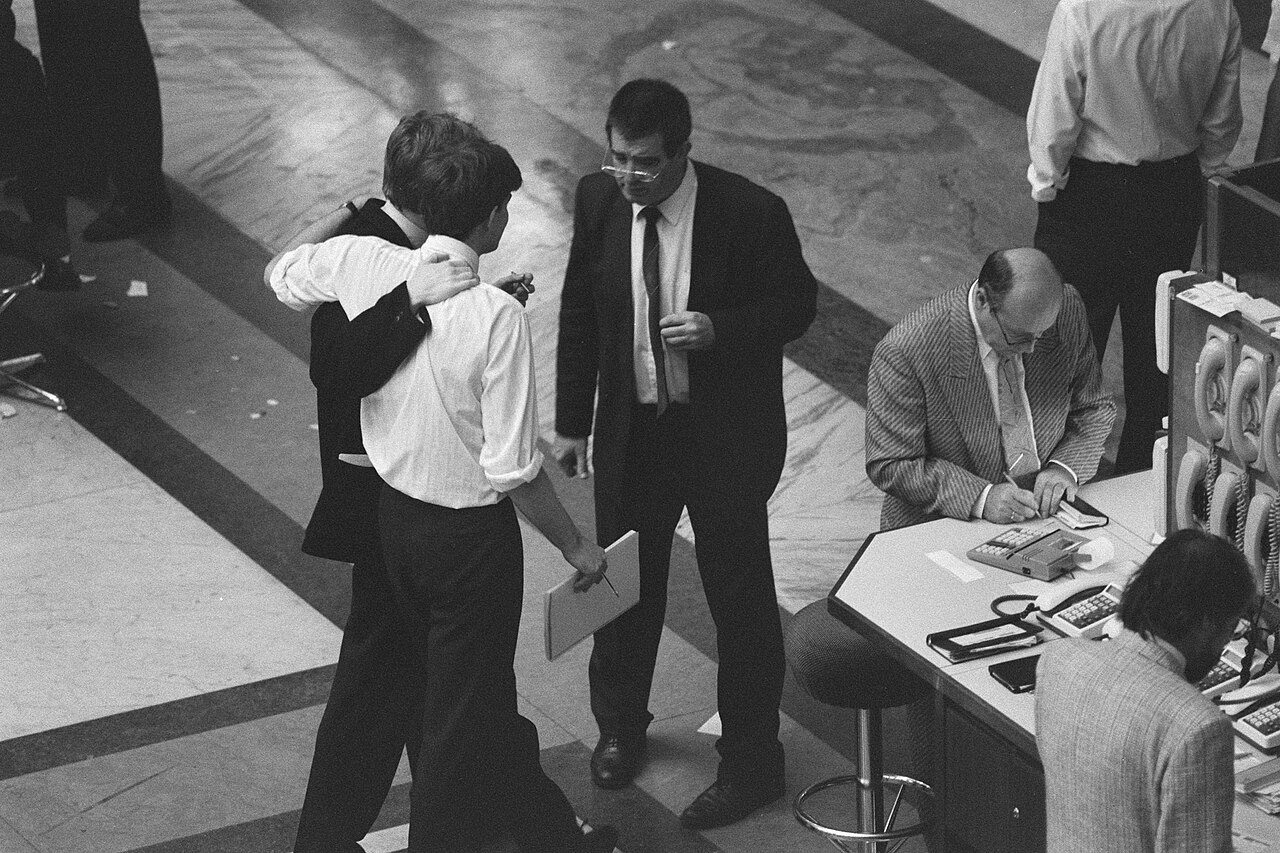
\includegraphics[height=0.36\textheight]{ch8_amsterdam_1987.jpg}\\[1mm]
\imgcap{Bursa din Amsterdam, 21 octombrie 1987, la două zile după crah}
\imgcredit{https://commons.wikimedia.org/wiki/File:Effectenbeurs_Amsterdam_na_koersval,_Bestanddeelnr_934-1094.jpg}{Foto: Bart Molendijk / Anefo (1987); CC0; Wikimedia Commons}
\end{column}
\end{columns}
\end{frame}

\begin{frame}{Volatilitatea: definiție și unități de măsură}
\itemsize{\small}
\begin{itemize}
    \item Randamentul logaritmic zilnic în \%: $r_t = 100\,(\ln P_t - \ln P_{t-1})$ (\sfmchlink{https://danpele.github.io/SFM/RO/Cursuri/capitol1_date_randamente_indicatori.pdf}{Capitolul 1})
    \begin{itemize}
        \item \textbf{volatilitatea} = abaterea standard a randamentelor, $\sigma = \sqrt{\mathrm{Var}(r_t)}$
        \item are unitatea de măsură a randamentului (\% pe zi); varianța $\sigma^2$ se măsoară în \%$^2$
    \end{itemize}
    \item \textbf{Anualizarea}: cu $a$ observații pe an și randamente necorelate, $\sigma_{\text{an}} = \sigma_{\text{zi}}\sqrt{a}$
    \begin{itemize}
        \item $a$ = frecvența reală: circa 252 pentru S\&P 500, 250 pentru BET, 365 pentru Bitcoin (tranzacționat în fiecare zi)
        \item regula $\sqrt{a}$ este regula rădăcinii pătrate a timpului din \sfmchlink{https://danpele.github.io/SFM/RO/Cursuri/capitol7_piete_eficiente_mers_aleator_vr.pdf}{Capitolul 7}: cere randamente necorelate
    \end{itemize}
    \item Volatilitatea măsoară dispersia în ambele sensuri: un cîștig mare contează la fel de mult ca o pierdere mare
    \begin{itemize}
        \item există și alte măsuri ale incertitudinii, de exemplu entropia informațională a randamentelor \refPeleA
    \end{itemize}
\end{itemize}
\end{frame}

\begin{frame}{Patru piețe, același tipar}
\itemsize{\footnotesize}
\begin{center}
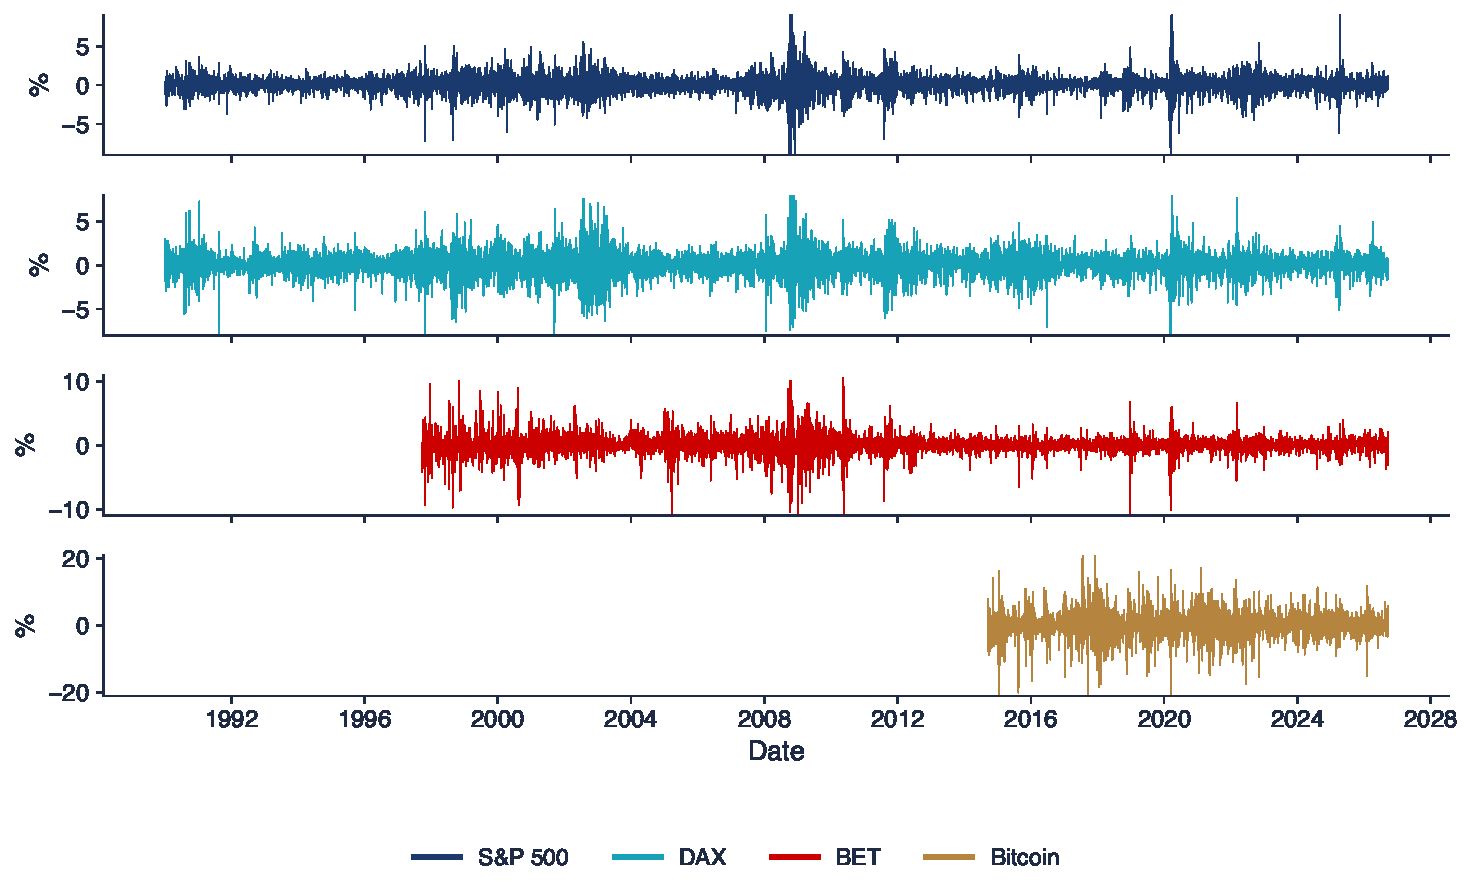
\includegraphics[width=0.97\textwidth,height=0.66\textheight,keepaspectratio]{sfm_ch8_returns_bursts.pdf}
\end{center}
\vspace{-0.25cm}
\begin{itemize}
    \item Randamente logaritmice zilnice în \%: S\&P 500 și DAX din 1990, BET din 1997, Bitcoin din 2014; ultima zi: 18 septembrie 2026
    \item Anii liniștiți alternează cu luni agitate în toate cele patru serii
\end{itemize}
\sfmquantlet{Ch_08}{SFM_ch8_returns_volatility}
\end{frame}

\begin{frame}{Interpretarea volatilității pe patru piețe}
\itemsize{\footnotesize}
\begin{center}
\footnotesize
\begin{tabular}{lrrrr}
\toprule
& \textbf{Volatilitate anuală} & \textbf{Cea mai mare variație zilnică} & \textbf{Data} & \textbf{Excesul de boltire} \\
\midrule
S\&P 500 & 18{,}0\% & ${-12{,}8}\%$ & 16 martie 2020 & 10{,}9 \\
DAX & 21{,}8\% & ${-13{,}1}\%$ & 12 martie 2020 & 6{,}0 \\
BET & 23{,}4\% & ${-13{,}1}\%$ & 7 ianuarie 2009 & 9{,}9 \\
Bitcoin & 66{,}6\% & ${-46{,}5}\%$ & 12 martie 2020 & 12{,}0 \\
\bottomrule
\end{tabular}
\end{center}
\begin{itemize}
    \item Bitcoin este cu circa 20\% mai volatil pe an decît ar rezulta dacă s-ar folosi greșit $\sqrt{252}$: se tranzacționează 365 de zile pe an
    \item Cele mai mari variații reprezintă 8--13 abateri standard: valori practic imposibile în cazul distribuției Normale (\sfmchlink{https://danpele.github.io/SFM/RO/Cursuri/capitol2_distributii_clasice_fapte_stilizate.pdf}{Capitolul 2})
    \item Excesul de boltire este mult peste 0 (valoarea pentru distribuția Normală): cozi groase; secțiunea 6 arată că volatility clustering este una dintre cauze
\end{itemize}\sfmquantlet{Ch_08}{SFM_ch8_returns_volatility}
\end{frame}

\begin{frame}{Volatilitatea este latentă}
\itemsize{\small}
\begin{itemize}
    \item Model: $r_t = \mu + \sigma_t z_t$, cu $z_t$ i.i.d., de medie 0 și varianță 1
    \begin{itemize}
        \item $\sigma_t$ este \textbf{volatilitatea condiționată}: $\sigma_t^2 = \mathrm{Var}(r_t \mid \mathcal{F}_{t-1})$, cu $\mathcal{F}_{t-1}$ informația de la închiderea zilei $t-1$
        \item \textbf{volatilitatea necondiționată} $\sigma = \sqrt{\mathrm{Var}(r_t)}$ este nivelul ei mediu pe termen lung
    \end{itemize}
    \item \textbf{Latentă}: nu observăm niciodată $\sigma_t$, ci doar un randament pe zi
    \begin{itemize}
        \item $r_t^2$ este o măsură nedeplasată, dar foarte zgomotoasă, a lui $\sigma_t^2$ (cu $\mu = 0$): $E[r_t^2 \mid \mathcal{F}_{t-1}] = \sigma_t^2$
        \item o zi liniștită poate apărea într-o perioadă agitată, și invers
    \end{itemize}
    \item Trei moduri de a obține mai multă informație despre $\sigma_t$
    \begin{itemize}
        \item calculăm media pe multe zile (volatilitatea istorică, EWMA); folosim întreaga traiectorie a zilei (prețurile maxim și minim); folosim prețurile din timpul zilei (volatilitatea realizată)
    \end{itemize}
\end{itemize}
\end{frame}

\begin{frame}{Exemplu rezolvat: anualizarea volatilității}
\itemsize{\small}
\begin{itemize}
    \item S\&P 500 din 1990: abaterea standard zilnică $\hat\sigma = 1{,}13\%$, $a = 252$ de observații pe an
    \begin{itemize}
        \item $\hat\sigma_{\text{an}} = 1{,}13 \times \sqrt{252} = 1{,}13 \times 15{,}87 = 18{,}0\%$
    \end{itemize}
    \item Bitcoin din 2014: $\hat\sigma = 3{,}49\%$ pe zi, 7 zile pe săptămînă
    \begin{itemize}
        \item corect: $3{,}49 \times \sqrt{365} = 3{,}49 \times 19{,}11 = 66{,}6\%$
        \item greșit, cu convenția de la acțiuni: $3{,}49 \times \sqrt{252} = 55{,}3\%$
    \end{itemize}
    \item Pentru a compara active: anualizați fiecare serie cu propriul calendar, apoi comparați
\end{itemize}
\end{frame}

\begin{frame}{Recapitulare: volatilitatea: definiție și caracter latent}
\itemsize{\small}
\begin{itemize}
    \item Volatilitatea = abaterea standard a randamentelor; se anualizează cu $\sqrt{a}$, unde $a$ este numărul real de observații pe an
    \item Volatilitatea condiționată $\sigma_t$ variază în timp și nu este observată niciodată: o putem doar estima
    \item Toate piețele au perioade liniștite și perioade agitate
\end{itemize}
\end{frame}


%=============================================================================
\section{Volatilitatea istorică și alegerea ferestrei}
%=============================================================================

\begin{frame}{Volatilitatea istorică (pe fereastră mobilă)}
\itemsize{\small}
\begin{itemize}
    \item \textbf{Volatilitatea istorică} pe o fereastră cu ultimele $n$ zile:
    \begin{itemize}
        \item $\hat\sigma_t = \sqrt{\dfrac{1}{n-1}\sum_{j=0}^{n-1}(r_{t-j} - \bar r_t)^2}$, cu $\bar r_t$ media acelorași $n$ randamente
        \item \textbf{fereastră mobilă}: în fiecare zi intră cel mai nou randament și iese cel mai vechi
    \end{itemize}
    \item Varianta cu media zero: $\hat\sigma_t^2 = \frac{1}{n}\sum_{j=0}^{n-1} r_{t-j}^2$
    \begin{itemize}
        \item pentru datele zilnice media este foarte mică în raport cu $\sigma$ ($0{,}03\%$ față de $1{,}13\%$ la S\&P 500); dacă o fixăm la 0, eliminăm o estimare zgomotoasă
    \end{itemize}
    \item Ferestre uzuale: $n = 21$ (o lună), $63$ (un trimestru), $252$ (un an) de zile de tranzacționare
    \begin{itemize}
        \item fiecare $\hat\sigma_t$ se anualizează cu $\sqrt{a}$ și se reprezintă în ultima zi a ferestrei
    \end{itemize}
\end{itemize}
\end{frame}

\begin{frame}{S\&P 500: trei ferestre, trei răspunsuri}
\itemsize{\footnotesize}
\begin{center}
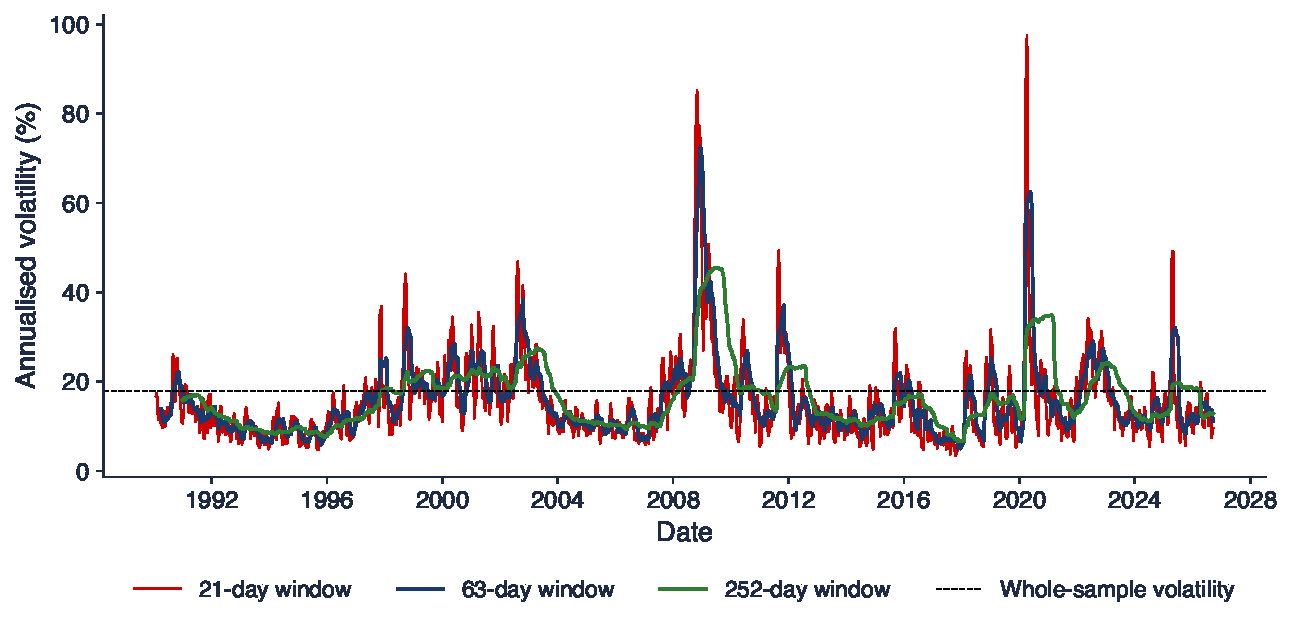
\includegraphics[width=0.97\textwidth,height=0.56\textheight,keepaspectratio]{sfm_ch8_rolling_windows.pdf}
\end{center}
\vspace{-0.25cm}
\begin{itemize}
    \item Volatilitatea S\&P 500 pe ferestre mobile, anualizată; linia punctată: volatilitatea pe întregul eșantion, 18{,}0\%
    \item \textbf{Întrebare pentru sală}: în ce fereastră ați avea încredere în ziua de după un crah?
\end{itemize}
\sfmquantlet{Ch_08}{SFM_ch8_returns_volatility}
\end{frame}

\begin{frame}{Interpretarea compromisului dintre ferestre}
\itemsize{\small}
\begin{itemize}
    \item Fereastra scurtă ($n = 21$): reacționează repede, dar este zgomotoasă
    \begin{itemize}
        \item maximul 97{,}5\% pe 6 aprilie 2020; variația zilnică tipică a lui $\ln\hat\sigma_t$ este 6{,}7\%
    \end{itemize}
    \item Fereastra lungă ($n = 252$): netedă, dar lentă
    \begin{itemize}
        \item maximul doar 45{,}6\%, atins pe 15 iulie 2009, la cîteva luni după vîrful crizei din 2008; variația zilnică 0{,}8\%
    \end{itemize}
    \item \textbf{Răspuns}: o fereastră scurtă sau EWMA (secțiunea următoare), deoarece media pe o fereastră lungă include încă zilele liniștite dinaintea crahului
    \begin{itemize}
        \item pentru planificarea capitalului se preferă o fereastră lungă: se schimbă lent
    \end{itemize}
    \item La sfîrșitul eșantionului: 9{,}6\% (21 de zile), 11{,}1\% (63 de zile), 12{,}9\% (252 de zile)
\end{itemize}\sfmquantlet{Ch_08}{SFM_ch8_returns_volatility}
\end{frame}

\begin{frame}{Precizia unei volatilități de selecție}
\itemsize{\small}
\begin{itemize}
    \item Cu $n$ randamente Normale i.i.d., eroarea standard relativă a lui $\hat\sigma$ este $\mathrm{SE}(\hat\sigma)/\sigma \approx 1/\sqrt{2n}$
    \begin{itemize}
        \item $n = 21$: 15\%; $n = 63$: 9\%; $n = 252$: 4\%
    \end{itemize}
    \item Cu cozi groase (coeficient de boltire $\kappa$): $\mathrm{SE}(\hat\sigma)/\sigma \approx \sqrt{(\kappa - 1)/(4n)}$ (metoda delta)
    \begin{itemize}
        \item S\&P 500: $\kappa = 13{,}9$, deci $n = 21$: 39\%; $n = 252$: 11\%
        \item pentru $\kappa = 3$ (distribuția Normală) cele două formule coincid
    \end{itemize}
    \item \textbf{Exemplu rezolvat}: ultima volatilitate pe 21 de zile a S\&P 500 este 9{,}6\%
    \begin{itemize}
        \item interval aproximativ de 95\%, randamente Normale: $[6{,}7\%; 12{,}5\%]$; cu boltirea observată: $[2{,}2\%; 17{,}0\%]$
    \end{itemize}
\end{itemize}
\end{frame}

\begin{frame}{Recapitulare: volatilitatea istorică}
\itemsize{\small}
\begin{itemize}
    \item Abaterea standard pe o fereastră mobilă de $n$ zile; pentru date zilnice media poate fi fixată la zero
    \item Ferestrele scurte reacționează repede, dar sînt zgomotoase; cele lungi sînt netede, dar lente
    \item O volatilitate pe 21 de zile are o incertitudine de $\pm$15\% sau mai mult: o zecimală înseamnă deja prea multă precizie
\end{itemize}
\end{frame}


%=============================================================================
\section{EWMA și RiskMetrics}
%=============================================================================

\begin{frame}{1994: RiskMetrics face din volatilitate o cifră zilnică}
\itemsize{\small}
\begin{columns}[T]
\begin{column}{0.56\textwidth}
\begin{itemize}
    \item J.P. Morgan a lansat RiskMetrics în octombrie 1994 și a publicat gratuit metodele și datele \refRM
    \begin{itemize}
        \item scopul: un etalon comun pentru riscul de piață, valabil pentru toate băncile
        \item volatilitățile și corelațiile a peste 480 de serii, actualizate zilnic
    \end{itemize}
    \item Metoda: o medie mobilă ponderată exponențial (EWMA) a randamentelor la pătrat
    \begin{itemize}
        \item un singur parametru, \textbf{factorul de atenuare} $\lambda$: $0{,}94$ pentru prognozele zilnice, $0{,}97$ pentru cele lunare
        \item pentru fiecare serie, $\lambda$ minimizează rădăcina erorii pătratice medii a prognozelor de varianță; 0,94 este media ponderată pe toate seriile
    \end{itemize}
\end{itemize}
\end{column}
\begin{column}{0.40\textwidth}
\centering
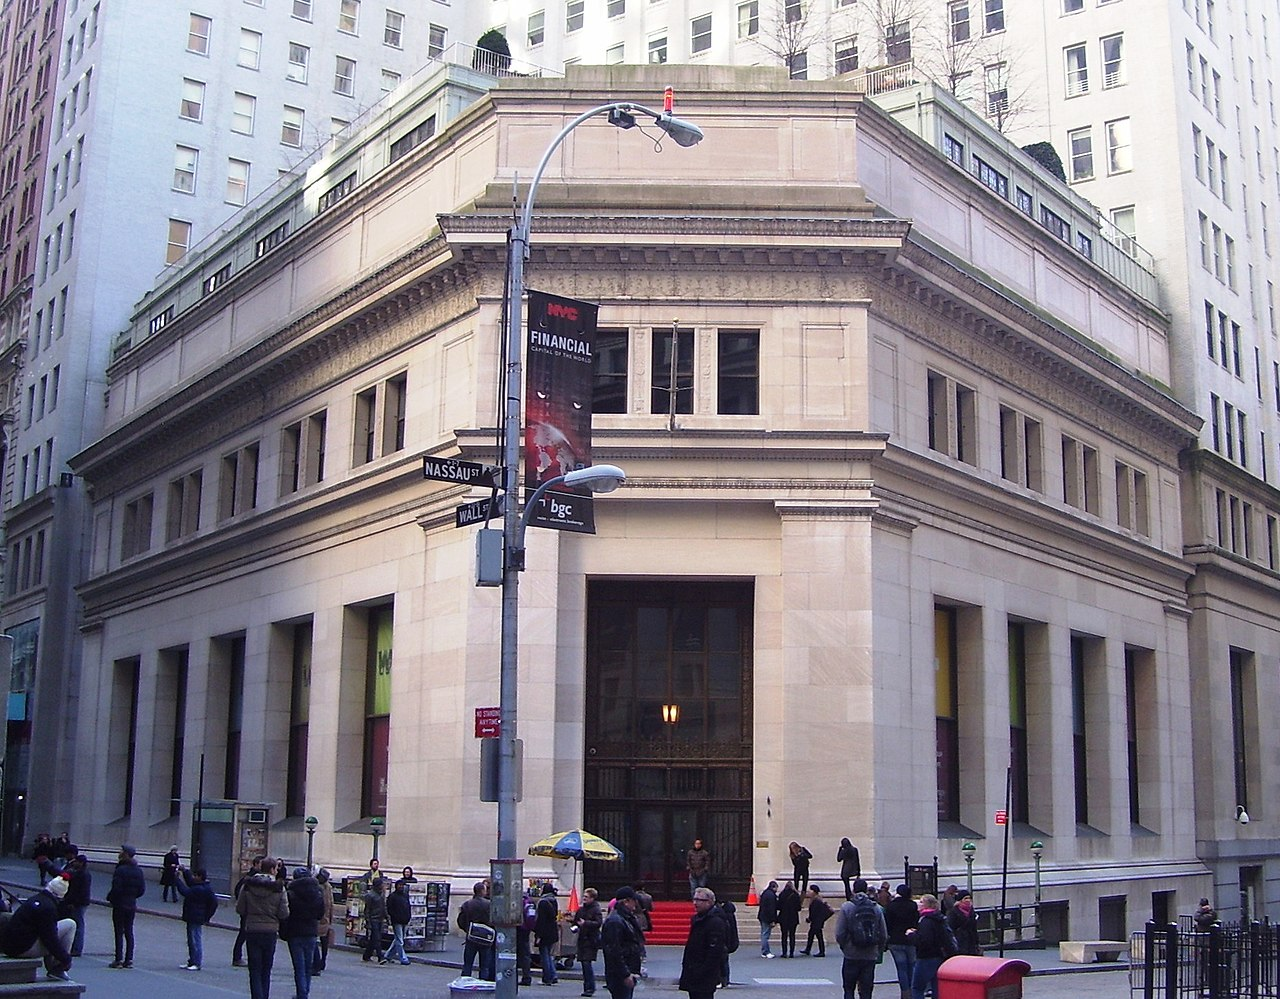
\includegraphics[height=0.38\textheight]{ch8_jpmorgan_23wall.jpg}\\[1mm]
\imgcap{Clădirea J.P. Morgan de la 23 Wall Street, New York}
\imgcredit{https://commons.wikimedia.org/wiki/File:J._P._Morgan_\%26_Company_Building_23_Wall_Street.jpg}{Foto: Beyond My Ken (2012); CC BY-SA 4.0; Wikimedia Commons}
\end{column}
\end{columns}
\end{frame}

\begin{frame}{Estimatorul EWMA}
\itemsize{\small}
\begin{itemize}
    \item Recurența \textbf{EWMA} (media zero): $\sigma_t^2 = \lambda\,\sigma_{t-1}^2 + (1-\lambda)\,r_{t-1}^2$, \ $0 < \lambda < 1$
    \begin{itemize}
        \item $\sigma_t^2$ folosește randamentele pînă în ziua $t-1$: este prognoza pentru ziua $t$
        \item valoarea inițială: $\sigma_1^2$ = media primelor randamente la pătrat; efectul ei dispare după cîteva luni
    \end{itemize}
    \item Prin dezvoltarea recurenței: $\sigma_t^2 = (1-\lambda)\sum_{j \ge 1}\lambda^{j-1} r_{t-j}^2$
    \begin{itemize}
        \item ponderile $(1-\lambda)\lambda^{j-1}$ scad geometric și au suma 1
        \item \textbf{timpul de înjumătățire}: decalajul la care ponderea se înjumătățește, $\ln 0{,}5/\ln\lambda$
    \end{itemize}
    \item O fereastră mobilă dă ponderea $1/n$ fiecăreia dintre ultimele $n$ zile și 0 tuturor zilelor mai vechi
\end{itemize}
\end{frame}

\begin{frame}{Ponderile EWMA față de ponderile unei ferestre mobile}
\itemsize{\footnotesize}
\begin{center}
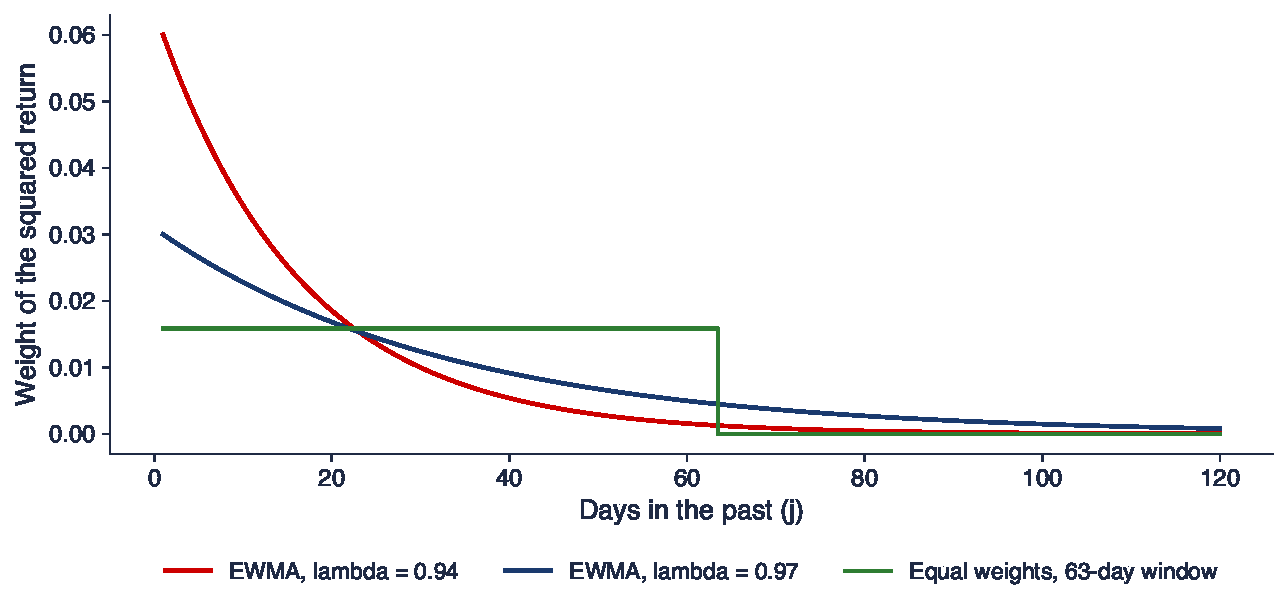
\includegraphics[width=0.97\textwidth,height=0.54\textheight,keepaspectratio]{sfm_ch8_ewma_weights.pdf}
\end{center}
\vspace{-0.25cm}
\begin{itemize}
    \item $\lambda = 0{,}94$: timp de înjumătățire 11{,}2 zile, decalaj mediu $1/(1-\lambda) = 16{,}7$ zile, 99\% din pondere în ultimele 74 de zile
    \item $\lambda = 0{,}97$: timp de înjumătățire 22{,}8 zile, 99\% din pondere în ultimele 151 de zile
\end{itemize}
\sfmquantlet{Ch_08}{SFM_ch8_ewma}
\end{frame}

\begin{frame}{Exemplu rezolvat: o actualizare EWMA}
\itemsize{\small}
\begin{itemize}
    \item Varianța EWMA de ieri: $\sigma_{t-1}^2 = 1{,}00$ (\%$^2$), adică o volatilitate zilnică de 1\%; randamentul de ieri: $r_{t-1} = -3\%$
    \begin{itemize}
        \item pasul 1: $\lambda\sigma_{t-1}^2 = 0{,}94 \times 1{,}00 = 0{,}94$
        \item pasul 2: $(1-\lambda)r_{t-1}^2 = 0{,}06 \times 9 = 0{,}54$
        \item pasul 3: $\sigma_t^2 = 0{,}94 + 0{,}54 = 1{,}48$, deci $\sigma_t = 1{,}22\%$ pe zi, $1{,}22 \times \sqrt{252} = 19{,}3\%$ pe an
    \end{itemize}
    \item Dacă ziua de azi este liniștită ($r_t = 0$): $\sigma_{t+1}^2 = 0{,}94 \times 1{,}48 = 1{,}39$
    \begin{itemize}
        \item șocul se atenuează cu 6\% pe zi; nu dispare niciodată brusc
    \end{itemize}
    \item O fereastră de 63 de zile ar adăuga azi $9/63 = 0{,}14$ la varianță și ar elimina dintr-odată această contribuție după 63 de zile
\end{itemize}
\end{frame}

\begin{frame}{Ghost effect: martie--iunie 2020}
\itemsize{\footnotesize}
\begin{center}
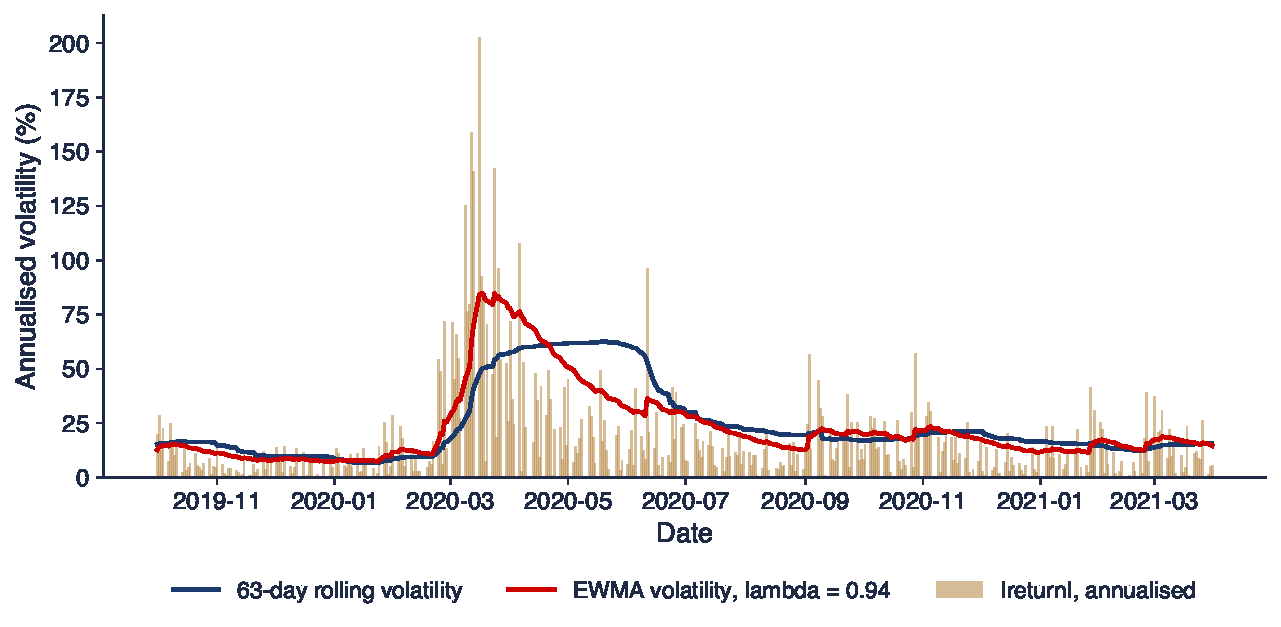
\includegraphics[width=0.97\textwidth,height=0.54\textheight,keepaspectratio]{sfm_ch8_ghost.pdf}
\end{center}
\vspace{-0.25cm}
\begin{itemize}
    \item S\&P 500: volatilitatea pe fereastra mobilă de 63 de zile și volatilitatea EWMA ($\lambda = 0{,}94$), anualizate; barele: $|r_t|$ pe aceeași scală anuală
    \item \textbf{Întrebare pentru sală}: de ce scade brusc linia albastră la mijlocul lui iunie 2020, într-o zi liniștită?
\end{itemize}
\sfmquantlet{Ch_08}{SFM_ch8_ewma}
\end{frame}

\begin{frame}{Interpretarea ghost effect}
\itemsize{\small}
\begin{itemize}
    \item \textbf{Răspuns}: pe 15 iunie 2020, randamentul din 16 martie 2020 ($-12{,}8\%$) a ieșit din fereastra de 63 de zile
    \begin{itemize}
        \item volatilitatea pe fereastra mobilă a scăzut de la 50{,}4\% la 43{,}0\% într-o singură zi, fără nicio știre
        \item acest artefact este \textbf{ghost effect}: un șoc vechi iese brusc din fereastră
    \end{itemize}
    \item EWMA reacționează mai repede și uită treptat
    \begin{itemize}
        \item vîrful EWMA: 84{,}8\% pe 24 martie 2020; vîrful pe 63 de zile: 62{,}6\% abia pe 20 mai 2020
        \item în ziua ghost effect, EWMA s-a modificat cu doar $-0{,}9$ puncte procentuale
    \end{itemize}
    \item Prețul vitezei: EWMA este mai zgomotos decît o fereastră lungă și nu are un nivel de lungă durată spre care să revină
\end{itemize}\sfmquantlet{Ch_08}{SFM_ch8_ewma}
\end{frame}

\begin{frame}{EWMA și GARCH: trimitere la \sfmchlinkt{https://danpele.github.io/SFM/RO/Cursuri/capitol9_modele_arch_garch.pdf}{Capitolul 9}}
\itemsize{\small}
\begin{itemize}
    \item \textbf{ARCH} \refEngle{} și \textbf{GARCH} \refBollerslev: $\sigma_t^2 = \omega + \alpha\, r_{t-1}^2 + \beta\,\sigma_{t-1}^2$
    \begin{itemize}
        \item EWMA este cazul particular $\omega = 0$, $\alpha = 1 - \lambda$, $\beta = \lambda$, deci $\alpha + \beta = 1$ (GARCH „integrat”, \textbf{IGARCH})
    \end{itemize}
    \item Consecințe pentru prognozele făcute în ziua $t$ pentru ziua $t + h$
    \begin{itemize}
        \item EWMA: constantă, $E_t[\sigma_{t+h}^2] = \sigma_{t+1}^2$ pentru orice $h$: nivelul de azi persistă la nesfîrșit
        \item GARCH cu $\alpha + \beta < 1$: atrasă spre varianța de lungă durată $\omega/(1 - \alpha - \beta)$
    \end{itemize}
    \item \sfmchlink{https://danpele.github.io/SFM/RO/Cursuri/capitol9_modele_arch_garch.pdf}{Capitolul 9} estimează $\omega$, $\alpha$, $\beta$ prin verosimilitate maximă; aici $\lambda$ este fixat sau ales după un criteriu de prognoză (secțiunea 8)
\end{itemize}
\end{frame}

\begin{frame}{Recapitulare: EWMA și RiskMetrics}
\itemsize{\small}
\begin{itemize}
    \item $\sigma_t^2 = \lambda\sigma_{t-1}^2 + (1-\lambda)r_{t-1}^2$; RiskMetrics: $\lambda = 0{,}94$ pentru date zilnice
    \item Ponderi geometrice: timp de înjumătățire 11{,}2 zile pentru $\lambda = 0{,}94$; fără ghost effect
    \item EWMA = IGARCH(1,1) fără constantă: prognoze constante, fără revenire la medie
\end{itemize}
\end{frame}


%=============================================================================
\section{Estimatori de amplitudine (range-based)}
%=============================================================================

\begin{frame}{Prețurile de deschidere, maxim, minim și închidere}
\itemsize{\small}
\begin{itemize}
    \item Datele \textbf{OHLC}: pentru fiecare zi $t$, deschiderea $O_t$, maximul $H_t$, minimul $L_t$ și închiderea $C_t$
    \begin{itemize}
        \item randamentul închidere--închidere folosește 2 prețuri pe zi; $H_t$ și $L_t$ conțin informație despre întreaga traiectorie a zilei
    \end{itemize}
    \item Notații (diferențe logaritmice în \%), fiecare față de deschiderea zilei $t$:
    \begin{itemize}
        \item $u_t = \ln(H_t/O_t)$, $d_t = \ln(L_t/O_t)$, $c_t = \ln(C_t/O_t)$; deci $d_t \le 0 \le u_t$ și $d_t \le c_t \le u_t$
        \item randamentul \textbf{overnight} $o_t = \ln(O_t/C_{t-1})$; randamentul zilnic este $r_t = o_t + c_t$
        \item \textbf{amplitudinea} (range) $u_t - d_t = \ln(H_t/L_t)$
    \end{itemize}
    \item Date: S\&P 500 din 2008, DAX din 2006, Bitcoin din 2014, acțiuni BVB din 2010; fișierul BET conține doar închideri
\end{itemize}
\end{frame}

\begin{frame}{O zi de tranzacționare: ce înregistrează OHLC}
\itemsize{\footnotesize}
\begin{center}
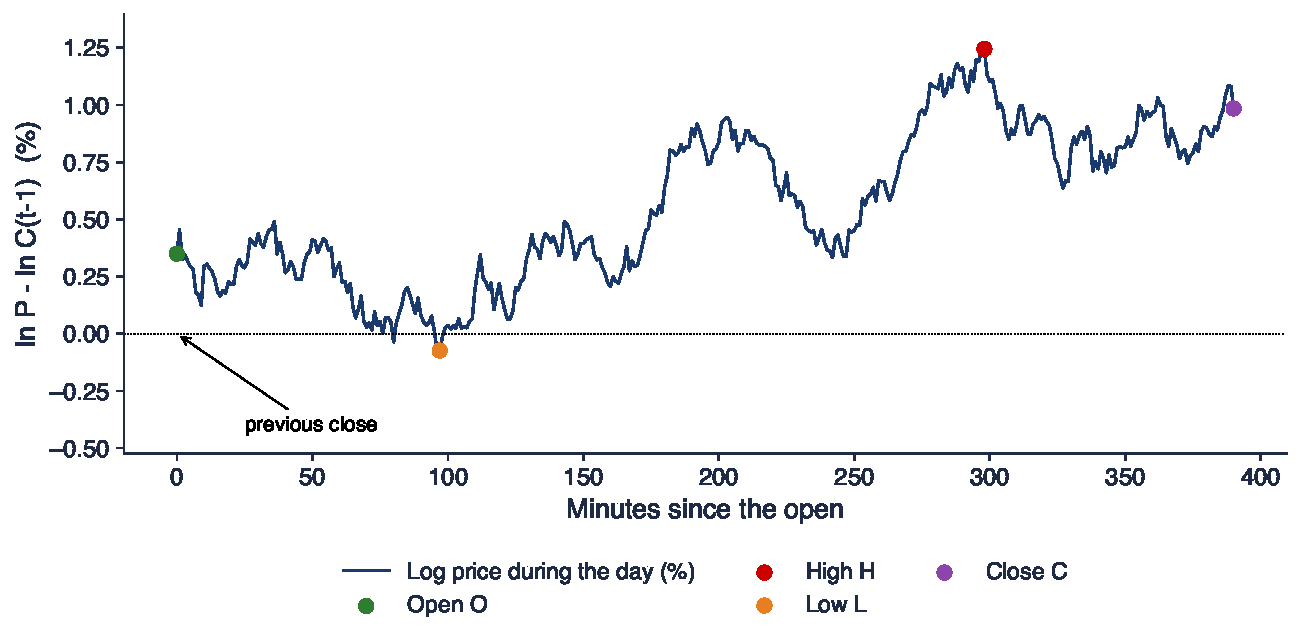
\includegraphics[width=0.97\textwidth,height=0.54\textheight,keepaspectratio]{sfm_ch8_ohlc_path.pdf}
\end{center}
\vspace{-0.25cm}
\begin{itemize}
    \item Preț logaritmic simulat (mișcare browniană, 390 de pași de un minut) după un salt overnight de $0{,}35\%$: închiderea păstrează doar punctul final; maximul și minimul rezumă traiectoria
    \item Două zile cu aceeași închidere pot avea amplitudini foarte diferite, deci riscuri foarte diferite
\end{itemize}
\sfmquantlet{Ch_08}{SFM_ch8_range_estimators}
\end{frame}

\begin{frame}{Estimatorul Parkinson (1980)}
\itemsize{\small}
\begin{itemize}
    \item Pentru o mișcare browniană fără tendință (drift), cu varianța $\sigma^2$ pe zi: $E[(u_t - d_t)^2] = 4\ln 2\;\sigma^2$ \refParkinson
    \begin{itemize}
        \item o zi: $\hat\sigma_{P,t}^2 = \dfrac{(u_t - d_t)^2}{4\ln 2}$; pe $n$ zile: media acestor valori
        \item $4\ln 2 \approx 2{,}77$: amplitudinea este, în medie, mai mare decît $\sigma$
    \end{itemize}
    \item Ipoteze
    \begin{itemize}
        \item tranzacționare continuă în timpul zilei, deci maximul și minimul observate sînt extremele reale
        \item fără tendință și fără salt overnight: amplitudinea vede doar ședința de tranzacționare
    \end{itemize}
    \item Mult mai precis decît $r_t^2$: o simulare din această secțiune măsoară cu cît
    \begin{itemize}
        \item logaritmul amplitudinii se folosește și la estimarea modelelor de volatilitate stochastică \refABD
    \end{itemize}
\end{itemize}
\end{frame}

\begin{frame}{Garman--Klass (1980) și Rogers--Satchell (1991)}
\itemsize{\small}
\begin{itemize}
    \item \textbf{Garman--Klass} \refGK: adaugă randamentul deschidere--închidere
    \begin{itemize}
        \item $\hat\sigma_{GK,t}^2 = 0{,}5\,(u_t - d_t)^2 - (2\ln 2 - 1)\,c_t^2$
        \item ponderile fac estimatorul nedeplasat și aproape de varianță minimă printre astfel de forme pătratice, în absența tendinței
    \end{itemize}
    \item \textbf{Rogers--Satchell} \refRS: nedeplasat pentru orice tendință $\mu$
    \begin{itemize}
        \item $\hat\sigma_{RS,t}^2 = u_t(u_t - c_t) + d_t(d_t - c_t)$
        \item util pentru active cu o tendință puternică pe fereastră (de exemplu, Bitcoin într-o perioadă de creștere puternică)
    \end{itemize}
    \item Ambele ignoră totuși randamentul overnight $o_t$: măsoară doar varianța ședinței de tranzacționare
\end{itemize}
\end{frame}

\begin{frame}{Yang--Zhang (2000): adăugarea nopții}
\itemsize{\small}
\begin{itemize}
    \item Pe o fereastră de $n$ zile \refYZ:
    \begin{itemize}
        \item $\hat\sigma_{YZ}^2 = \hat\sigma_O^2 + k\,\hat\sigma_C^2 + (1-k)\,\hat\sigma_{RS}^2$, \quad $k = \dfrac{0{,}34}{1{,}34 + (n+1)/(n-1)}$
        \item $\hat\sigma_O^2$, $\hat\sigma_C^2$: varianțele de selecție ale randamentelor overnight $o_t$ și ale randamentelor deschidere--închidere $c_t$; $\hat\sigma_{RS}^2$: media termenului Rogers--Satchell
    \end{itemize}
    \item Proprietăți
    \begin{itemize}
        \item nedeplasat cu tendință și cu salturi la deschidere; $k$ minimizează varianța estimatorului
        \item $n = 21$: $k = 0{,}34/(1{,}34 + 22/20) = 0{,}34/2{,}44 = 0{,}14$
    \end{itemize}
    \item Cere o fereastră de $n \ge 2$ zile (varianțe de selecție); Parkinson, Garman--Klass și Rogers--Satchell funcționează și pentru o singură zi
\end{itemize}
\end{frame}

\begin{frame}{Exemplu rezolvat: S\&P 500 pe 16 martie 2020}
\itemsize{\small}
\begin{itemize}
    \item Închiderea precedentă 2\,711; deschiderea 2\,509, maximul 2\,563, minimul 2\,381, închiderea 2\,386
    \begin{itemize}
        \item $o = -7{,}76$, $u = 2{,}14$, $d = -5{,}22$, $c = -5{,}00$ (în \%); închidere--închidere $r = o + c = -12{,}77$
    \end{itemize}
    \item Estimări ale varianței pentru o zi (\%$^2$)
    \begin{itemize}
        \item închidere--închidere: $r^2 = 163{,}0$
        \item Parkinson: $(7{,}37)^2/2{,}773 = 19{,}6$; Garman--Klass: 17{,}5; Rogers--Satchell: 16{,}5
        \item partea overnight $o^2 = 60{,}2$; overnight plus Rogers--Satchell: 76{,}7
    \end{itemize}
    \item Cea mai mare parte a scăderii s-a produs overnight, înainte de deschidere: estimatorii care ignoră $o_t$ ratează cea mai mare parte a riscului din această zi
\end{itemize}\sfmquantlet{Ch_08}{SFM_ch8_range_estimators}
\end{frame}

\begin{frame}{Eficiența estimatorilor prin simulare}
\itemsize{\footnotesize}
\begin{center}
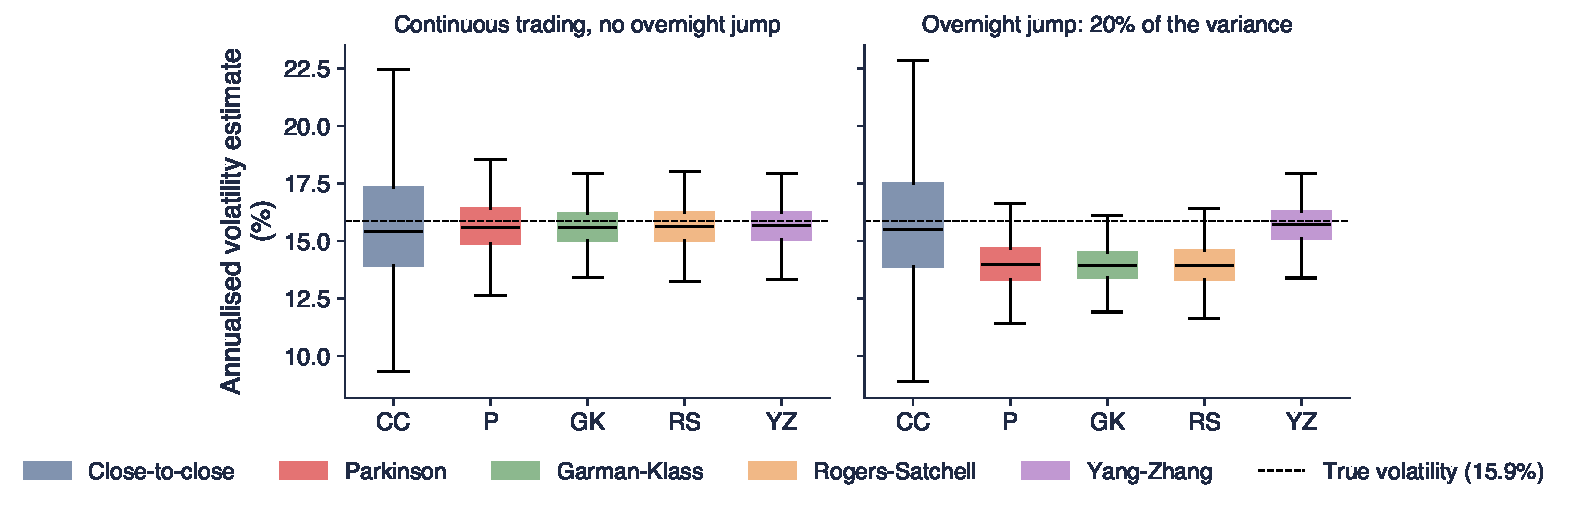
\includegraphics[width=0.97\textwidth,height=0.52\textheight,keepaspectratio]{sfm_ch8_efficiency.pdf}
\end{center}
\vspace{-0.25cm}
\begin{itemize}
    \item 1000 de ferestre de 21 de zile; volatilitatea reală $1\%$ pe zi ($15{,}9\%$ pe an); mișcare browniană intrazilnică pe 4680 de pași (unul la 5 secunde)
    \item \textbf{Eficiența} unui estimator: $\mathrm{Var}(\hat\sigma^2_{CC})/\mathrm{Var}(\hat\sigma^2)$, CC fiind estimatorul închidere--închidere; panoul din dreapta: 20\% din varianța zilnică apare overnight
\end{itemize}
\sfmquantlet{Ch_08}{SFM_ch8_range_efficiency}
\end{frame}

\begin{frame}{Interpretarea simulării: precizie și deplasare}
\itemsize{\footnotesize}
\begin{center}
\footnotesize
\begin{tabular}{lrrrrr}
\toprule
& \textbf{CC} & \textbf{Parkinson} & \textbf{GK} & \textbf{RS} & \textbf{YZ} \\
\midrule
Eficiența, tranzacționare continuă & 1{,}0 & 5{,}4 & 9{,}3 & 7{,}6 & 8{,}5 \\
Deplasarea (\%), tranzacționare continuă & ${0}$ & ${-2}$ & ${-3}$ & ${-3}$ & ${-2}$ \\
Deplasarea (\%), salt overnight & ${1}$ & ${-22}$ & ${-22}$ & ${-22}$ & ${-2}$ \\
Raportul MSE, salt overnight & 1{,}0 & 1{,}8 & 1{,}8 & 1{,}8 & 9{,}0 \\
Deplasarea (\%), 26 de prețuri pe zi & ${0}$ & ${-23}$ & ${-32}$ & ${-32}$ & ${-28}$ \\
\bottomrule
\end{tabular}
\end{center}
\begin{itemize}
    \item Cu tranzacționare continuă, estimatorii de amplitudine sînt de 5--9 ori mai eficienți: o lună de amplitudini conține tot atîta informație cît 5--9 luni de închideri
    \item Cu salt overnight, Parkinson, GK și RS ratează noaptea (deplasare de circa $-22\%$); doar YZ rămîne nedeplasat; raportul \textbf{MSE} (mean squared error, eroarea pătratică medie) = $\mathrm{MSE}(CC)/\mathrm{MSE}$
    \item Cu puține tranzacții amplitudinea observată este prea mică: toți estimatorii de amplitudine subestimează (piețe puțin lichide) \refMolnar
\end{itemize}\sfmquantlet{Ch_08}{SFM_ch8_range_efficiency}
\end{frame}

\begin{frame}{Date reale: cinci estimatori, cinci active}
\itemsize{\footnotesize}
\begin{center}
\footnotesize
\begin{tabular}{lrrrrrrrr}
\toprule
& \textbf{Din} & \textbf{CC} & \textbf{P} & \textbf{GK} & \textbf{RS} & \textbf{YZ} & \textbf{Ponderea nopții} & $\mathrm{corr}(o, c)$ \\
\midrule
S\&P 500 & 2008 & 19{,}9 & 15{,}4 & 14{,}6 & 14{,}4 & 16{,}3 & 13\% & ${0{,}22}$ \\
DAX & 2006 & 20{,}9 & 16{,}7 & 16{,}6 & 16{,}6 & 20{,}3 & 31\% & ${0{,}02}$ \\
Bitcoin & 2014 & 66{,}6 & 63{,}5 & 62{,}4 & 62{,}5 & 63{,}2 & 0\% & ${0{,}02}$ \\
TLV & 2010 & 26{,}6 & 21{,}5 & 20{,}6 & 21{,}0 & 25{,}6 & 26\% & ${-0{,}08}$ \\
SNP & 2010 & 24{,}5 & 21{,}4 & 20{,}8 & 21{,}4 & 25{,}8 & 27\% & ${-0{,}20}$ \\
\bottomrule
\end{tabular}
\end{center}
\begin{itemize}
    \item Volatilitatea anualizată (\%) pe întregul eșantion OHLC; P = Parkinson; ponderea nopții $= \hat\sigma_O^2/(\hat\sigma_O^2 + \hat\sigma_C^2)$
    \item Acțiuni: deschiderea, maximul și minimul ajustate cu același factor ca închiderea; zilele fără tranzacții sînt eliminate
\end{itemize}\sfmquantlet{Ch_08}{SFM_ch8_range_estimators}
\end{frame}

\begin{frame}{Interpretarea diferențelor dintre estimatori}
\itemsize{\small}
\begin{itemize}
    \item Bitcoin se tranzacționează 24 de ore din 24: ponderea nopții este aproape 0, iar toți cei cinci estimatori sînt apropiați
    \begin{itemize}
        \item diferența rămasă: traiectoria zilei este observată prin tranzacții discrete, nu continuu
    \end{itemize}
    \item DAX și acțiunile BVB: între un sfert și o treime din varianță apare overnight
    \begin{itemize}
        \item Parkinson, GK și RS sînt mult sub CC; YZ, care adaugă noaptea, este apropiat de CC
    \end{itemize}
    \item S\&P 500: chiar și YZ (16{,}3\%) rămîne sub CC (19{,}9\%)
    \begin{itemize}
        \item randamentele overnight și cele deschidere--închidere sînt corelate pozitiv (0{,}22); o explicație probabilă: deschiderea indicelui folosește prețuri vechi ale acțiunilor care încă nu s-au tranzacționat
        \item $\mathrm{Var}(r) = \mathrm{Var}(o) + \mathrm{Var}(c) + 2\,\mathrm{Cov}(o, c)$: niciun estimator de amplitudine nu vede termenul de covarianță
    \end{itemize}
    \item Lecția: verificați ipotezele pe date înainte de a avea încredere într-un cîștig de eficiență
\end{itemize}\sfmquantlet{Ch_08}{SFM_ch8_range_estimators}
\end{frame}

\begin{frame}{S\&P 500: estimări pe 21 de zile din 2019}
\itemsize{\footnotesize}
\begin{center}
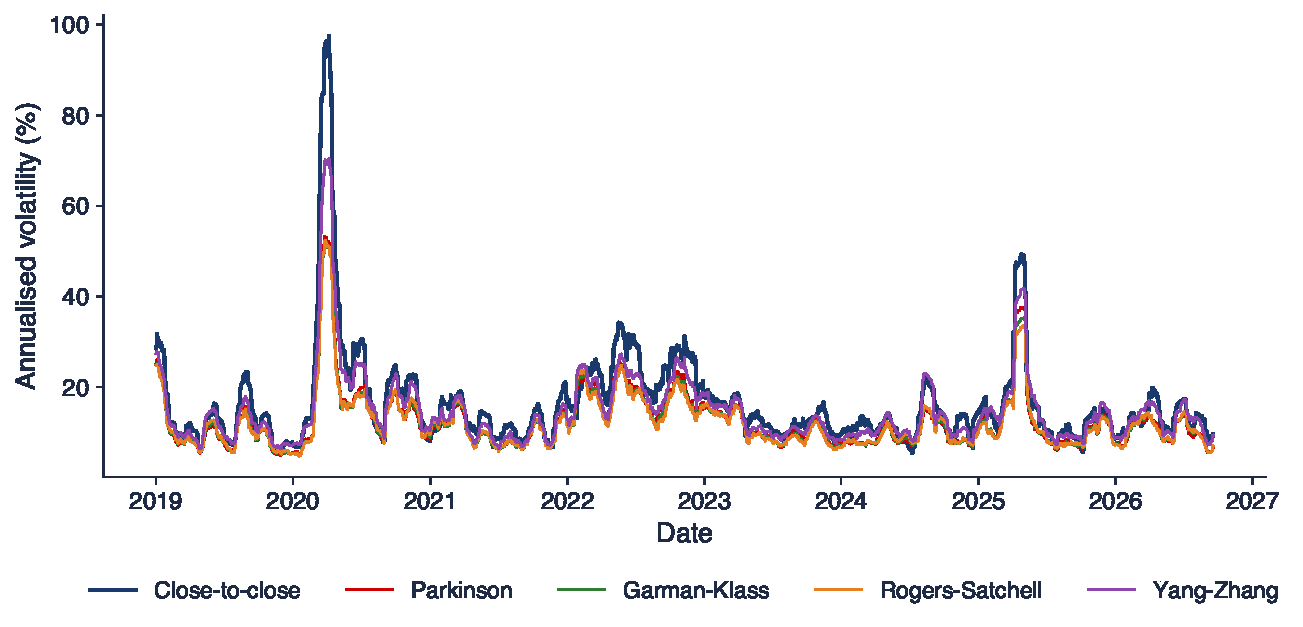
\includegraphics[width=0.97\textwidth,height=0.54\textheight,keepaspectratio]{sfm_ch8_range_rolling.pdf}
\end{center}
\vspace{-0.25cm}
\begin{itemize}
    \item Volatilitatea pe 21 de zile, anualizată, calculată cu cei cinci estimatori; medii din 2019: CC 16{,}3\%, Parkinson 12{,}5\%, YZ 14{,}7\%
    \item Liniile estimatorilor de amplitudine sînt mai netede: variația zilnică tipică a estimării logaritmice este 4{,}3\% pentru Parkinson și 4{,}2\% pentru YZ, față de 7{,}1\% pentru CC
\end{itemize}
\sfmquantlet{Ch_08}{SFM_ch8_range_estimators}
\end{frame}

\begin{frame}{Recapitulare: estimatori de amplitudine}
\itemsize{\small}
\begin{itemize}
    \item Parkinson folosește amplitudinea, Garman--Klass adaugă randamentul deschidere--închidere, Rogers--Satchell permite o tendință, Yang--Zhang adaugă noaptea
    \item În teorie de 5--9 ori mai eficienți decît estimatorul închidere--închidere; în practică deplasați în jos de salturile overnight și de tranzacționarea discretă
    \item Alegeți Yang--Zhang pentru piețele care se închid noaptea; orice estimator de amplitudine pentru piețele deschise 24 de ore
\end{itemize}
\end{frame}


%=============================================================================
\section{Volatilitatea realizată}
%=============================================================================

\begin{frame}{Varianța realizată din randamentele intrazilnice}
\itemsize{\small}
\begin{itemize}
    \item Împărțim ziua $t$ în $M$ intervale (de exemplu $M = 78$ de randamente de cinci minute $r_{t,i}$ într-o ședință de 6,5 ore)
    \begin{itemize}
        \item \textbf{varianța realizată} $\mathrm{RV}_t = \sum_{i=1}^{M} r_{t,i}^2$; \textbf{volatilitatea realizată} $= \sqrt{\mathrm{RV}_t}$
        \item cînd $M \to \infty$, $\mathrm{RV}_t$ converge către \textbf{varianța integrată} a zilei $t$, adică varianța reală a zilei \refABDL, \refBNS
    \end{itemize}
    \item Volatilitatea devine aproape observabilă: o măsură aproape fără eroare pentru fiecare zi
    \begin{itemize}
        \item se folosește la evaluarea prognozelor (secțiunea 8) și la prognoza directă a volatilității, de exemplu cu modelul HAR \refCorsi
        \item prețuri Bitcoin de înaltă frecvență și riscul zilnic: \refPeleB
    \end{itemize}
    \item Datele cursului sînt zilnice; următoarele două slide-uri folosesc prețuri simulate la un minut pentru a arăta comportamentul RV
\end{itemize}
\end{frame}

\begin{frame}{Exemplu simulat: RV urmărește volatilitatea reală}
\itemsize{\footnotesize}
\begin{center}
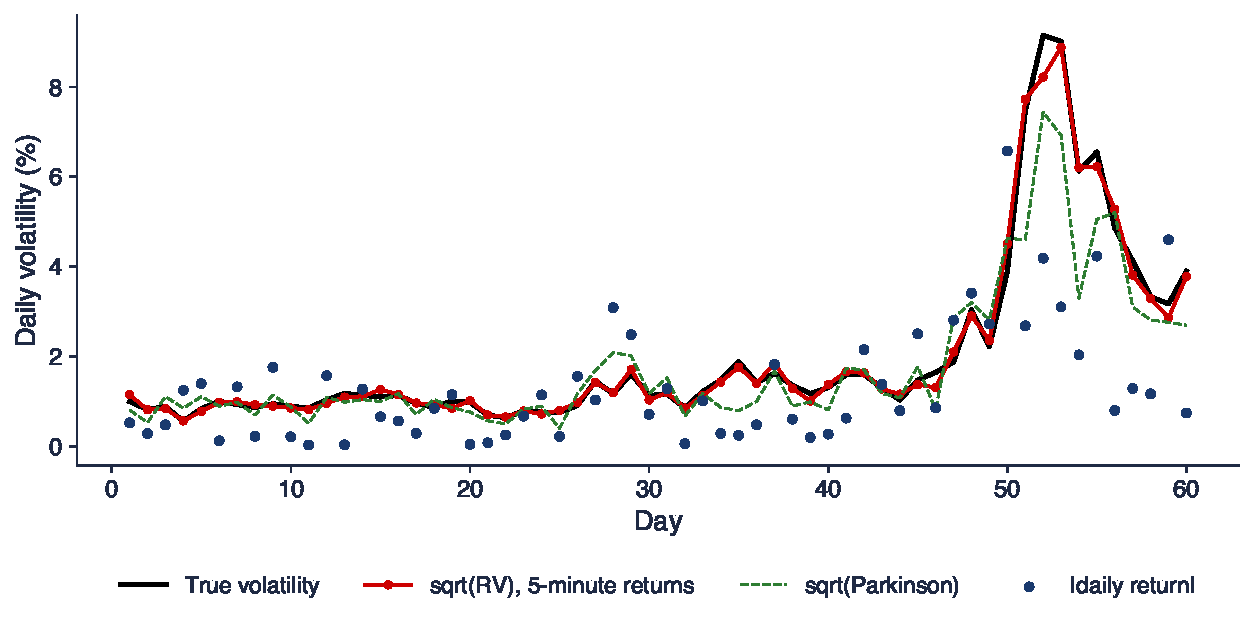
\includegraphics[width=0.97\textwidth,height=0.52\textheight,keepaspectratio]{sfm_ch8_realised.pdf}
\end{center}
\vspace{-0.25cm}
\begin{itemize}
    \item 60 de zile simulate, fiecare cu 390 de randamente de un minut; logaritmul volatilității zilnice urmează un proces AR(1) (persistența $0{,}9$)
    \item Eroarea relativă absolută medie: RV la 5 minute 6\%, Parkinson 23\%, $|r_t|$ 58\%; corelația cu valoarea reală: 0{,}995; 0{,}94 și 0{,}59
\end{itemize}
\sfmquantlet{Ch_08}{SFM_ch8_realised_volatility}
\end{frame}

\begin{frame}{Zgomotul de microstructură și signature plot}
\itemsize{\footnotesize}
\begin{center}
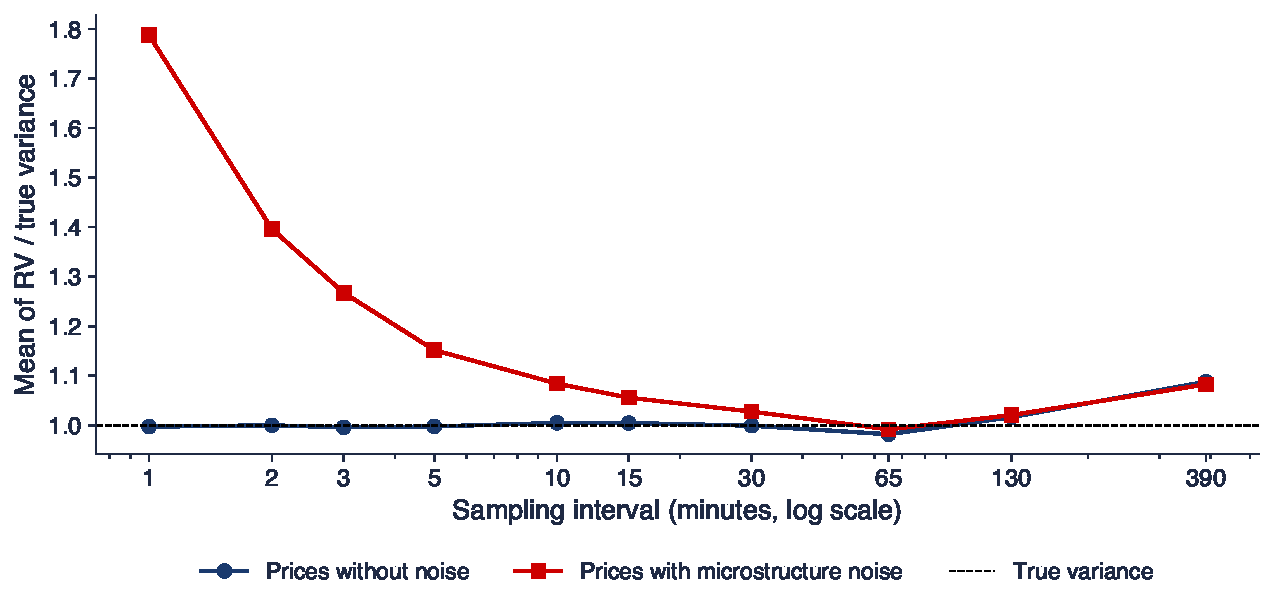
\includegraphics[width=0.97\textwidth,height=0.46\textheight,keepaspectratio]{sfm_ch8_signature.pdf}
\end{center}
\vspace{-0.25cm}
\begin{itemize}
    \item Prețurile observate = prețurile reale + \textbf{zgomot de microstructură} (oscilația între bid și ask, pasul de cotare), aici cu abaterea standard $0{,}025\%$; fiecare randament la pătrat crește atunci, în medie, cu dublul varianței zgomotului
    \item Cu zgomot, RV la un minut supraestimează varianța de 1{,}79 ori; la 5 minute: 1{,}15; \textbf{signature plot} arată RV în funcție de intervalul de eșantionare
    \item În practică, RV la 5 minute este greu de depășit \refLPS
\end{itemize}
\sfmquantlet{Ch_08}{SFM_ch8_realised_volatility}
\end{frame}

\begin{frame}{Recapitulare: volatilitatea realizată}
\itemsize{\small}
\begin{itemize}
    \item $\mathrm{RV}_t = \sum_i r_{t,i}^2$ estimează varianța unei zile aproape fără eroare
    \item Eșantionarea prea deasă preia zgomotul de microstructură; 5 minute este compromisul uzual
    \item Ordinea după precizie a măsurilor zilnice: RV $>$ estimatorii de amplitudine $>$ randamentul zilnic la pătrat
\end{itemize}
\end{frame}


%=============================================================================
\section{Volatility clustering}
%=============================================================================

\begin{frame}{1982: Engle și modelul ARCH}
\itemsize{\small}
\begin{columns}[T]
\begin{column}{0.60\textwidth}
\begin{itemize}
    \item \textbf{Volatility clustering}: perioadele cu randamente mari în valoare absolută alternează cu perioade cu randamente mici \refMandelbrot, \refCont
    \begin{itemize}
        \item randamentele sînt aproape necorelate (\sfmchlink{https://danpele.github.io/SFM/RO/Cursuri/capitol7_piete_eficiente_mers_aleator_vr.pdf}{Capitolul 7}), dar $|r_t|$ și $r_t^2$ sînt puternic autocorelate
    \end{itemize}
    \item Robert F. Engle \refEngle: varianța de azi depinde de șocurile la pătrat de ieri: \textbf{ARCH}
    \begin{itemize}
        \item primul model în care $\sigma_t$ variază în timp într-un mod previzibil
        \item Premiul Nobel pentru economie (2003), împărțit cu Clive Granger \refNobel; prelegerea Nobel a lui Engle: \refEngleN
    \end{itemize}
    \item Această secțiune: testele pentru volatility clustering; \sfmchlink{https://danpele.github.io/SFM/RO/Cursuri/capitol9_modele_arch_garch.pdf}{Capitolul 9}: modelele
\end{itemize}
\end{column}
\begin{column}{0.36\textwidth}
\centering

\includegraphics[height=0.40\textheight]{ch8_engle_2017.png}\\[1mm]
\imgcap{Robert F. Engle (n. 1942), Santiago, 2017}
\imgcredit{https://commons.wikimedia.org/wiki/File:Robert_Engle_SantiagoWEAI2017.png}{Foto: Econterms (2017); CC BY-SA 4.0; Wikimedia Commons}
\end{column}
\end{columns}
\end{frame}

\begin{frame}{Semnul este imprevizibil, mărimea nu}
\itemsize{\footnotesize}
\begin{center}
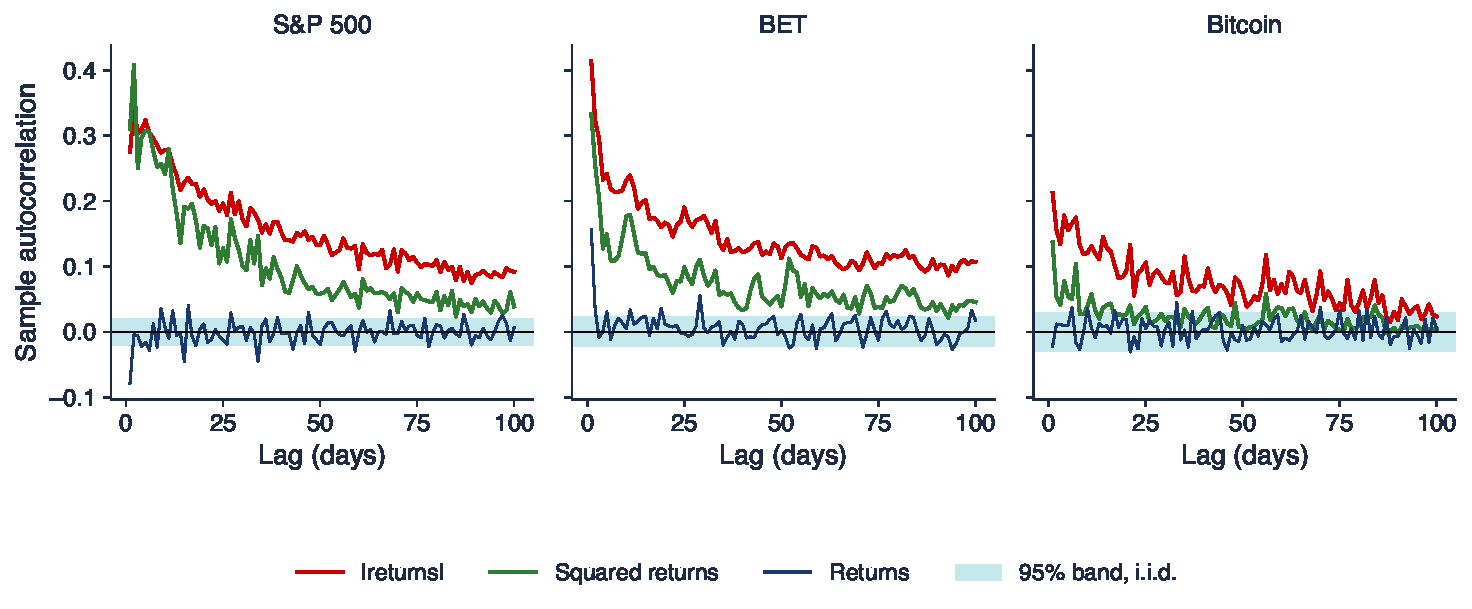
\includegraphics[width=0.97\textwidth,height=0.52\textheight,keepaspectratio]{sfm_ch8_acf_clustering.pdf}
\end{center}
\vspace{-0.25cm}
\begin{itemize}
    \item ACF de selecție (funcția de autocorelație, \sfmchlink{https://danpele.github.io/SFM/RO/Cursuri/capitol7_piete_eficiente_mers_aleator_vr.pdf}{Capitolul 7}) pentru $r_t$, $r_t^2$ și $|r_t|$, decalajele 1--100, cu banda de 95\% $\pm 1{,}96/\sqrt{T}$ pentru date i.i.d.
    \item S\&P 500: toate cele 100 de autocorelații ale lui $r_t^2$ și $|r_t|$ sînt deasupra benzii; la decalajul 100, $|r_t|$ are încă $0{,}09$
\end{itemize}
\sfmquantlet{Ch_08}{SFM_ch8_clustering}
\end{frame}

\begin{frame}{Interpretarea volatility clustering pe trei piețe}
\itemsize{\footnotesize}
\begin{center}
\footnotesize
\begin{tabular}{lrrrrrr}
\toprule
& $\hat\rho_1(|r|)$ & $\hat\rho_{10}(|r|)$ & $\hat\rho_{100}(|r|)$ & $\hat\rho_1(r^2)$ & $\hat\rho_{10}(r^2)$ & \textbf{Decalaje în afara benzii, $|r|$} \\
\midrule
S\&P 500 & $0{,}27$ & $0{,}28$ & $0{,}09$ & $0{,}31$ & $0{,}24$ & 100/100 \\
BET & $0{,}41$ & $0{,}23$ & $0{,}11$ & $0{,}33$ & $0{,}18$ & 100/100 \\
Bitcoin & $0{,}21$ & $0{,}12$ & $0{,}02$ & $0{,}14$ & $0{,}04$ & 92/100 \\
\bottomrule
\end{tabular}
\end{center}
\begin{itemize}
    \item Scădere lentă: un șoc de volatilitate se vede încă după luni de zile; Capitolul 11 numește acest fenomen memorie lungă
    \item \textbf{Efectul Taylor}: $|r_t|$ este mai autocorelat decît $r_t^2$ (96\% dintre decalaje la S\&P 500, toate decalajele la BET și Bitcoin) \refDGE
    \item Bitcoin: volatility clustering mai slab în $r_t^2$ (26 din 100 de decalaje în afara benzii): cîteva zile foarte mari domină pătratele
\end{itemize}\sfmquantlet{Ch_08}{SFM_ch8_clustering}
\end{frame}

\begin{frame}{Este volatility clustering real? Amestecați zilele}
\itemsize{\footnotesize}
\begin{center}
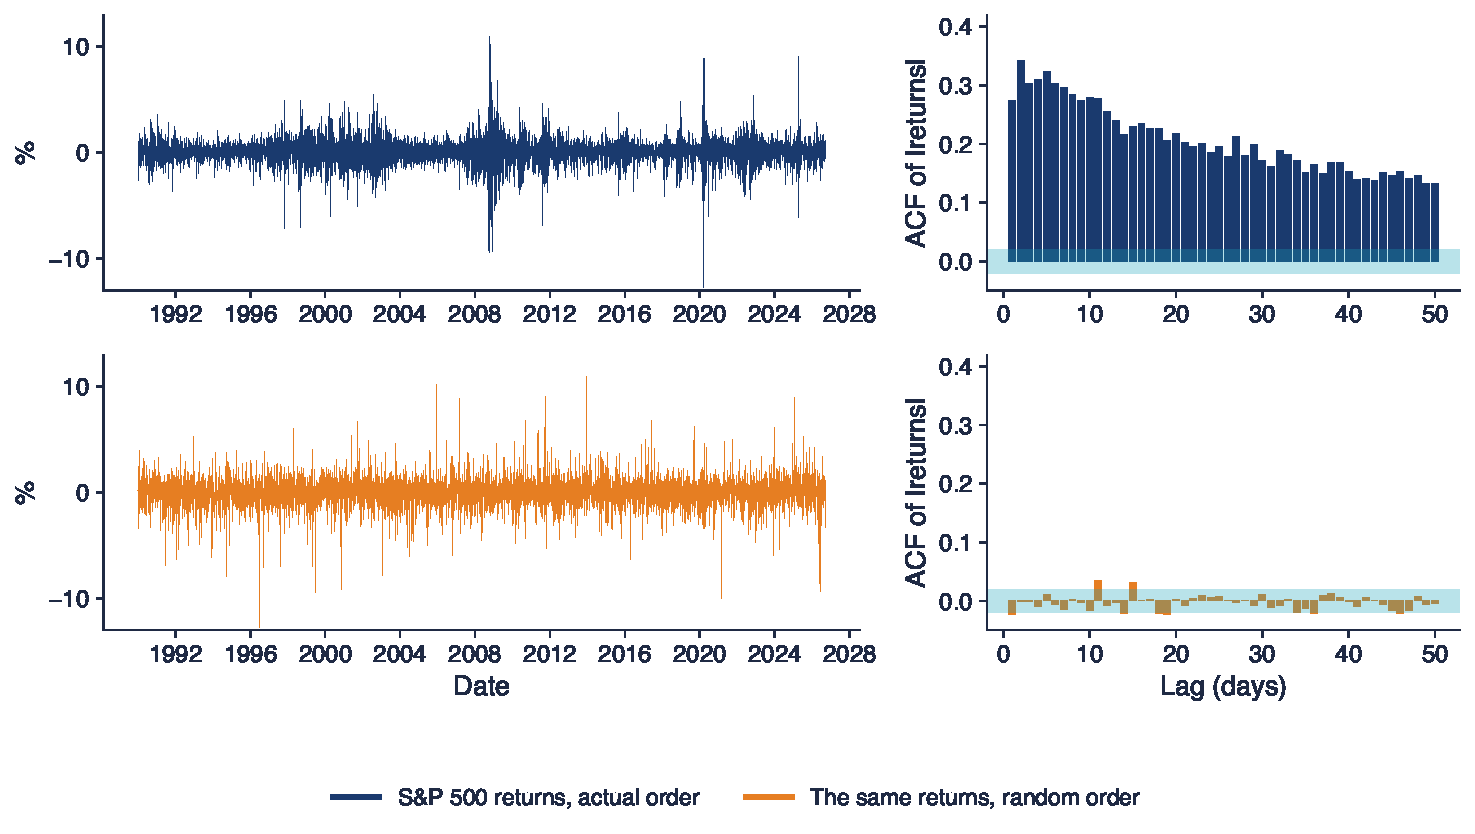
\includegraphics[width=0.97\textwidth,height=0.48\textheight,keepaspectratio]{sfm_ch8_shuffle.pdf}
\end{center}
\vspace{-0.25cm}
\begin{itemize}
    \item Aceleași randamente S\&P 500 într-o ordine aleatoare: aceeași distribuție și aceeași boltire (excesul de boltire 10{,}9), dar fără volatility clustering
    \item $\hat\rho_1(|r|)$: $0{,}27$ în ordinea reală, $-0{,}02$ după amestecare; Ljung--Box $Q(10)$ pentru $r_t^2$: 8\,015 față de 6{,}3
    \item Volatility clustering este o proprietate a \textbf{ordinii} randamentelor, nu a distribuției lor
\end{itemize}
\sfmquantlet{Ch_08}{SFM_ch8_clustering}
\end{frame}

\begin{frame}{Testarea volatility clustering: Ljung--Box pe randamentele la pătrat}
\itemsize{\small}
\begin{itemize}
    \item $H_0$: fără volatility clustering, $\mathrm{Var}(r_t \mid \mathcal{F}_{t-1})$ constantă, deci $r_t^2$ este necorelat
    \begin{itemize}
        \item \textbf{Testul McLeod--Li} \refML: statistica Ljung--Box \refLjung{} aplicată lui $r_t^2$
        \item $Q(m) = T(T+2)\sum_{k=1}^m \hat\rho_k(r^2)^2/(T-k) \sim \chi^2(m)$ în ipoteza $H_0$; respingem dacă $Q(m)$ depășește cuantila de 95\%
    \end{itemize}
    \item \textbf{Exemplu rezolvat}: S\&P 500, $T = 9\,240$, $m = 3$
    \begin{itemize}
        \item $\hat\rho_1, \hat\rho_2, \hat\rho_3$ pentru $r_t^2$: $0{,}311$; $0{,}408$; $0{,}250$
        \item termenii $T(T+2)\hat\rho_k^2/(T-k)$: 892; 1\,540; 579; $Q(3) = 3\,012 \gg \chi^2_{0{,}95}(3) = 7{,}81$: respingem $H_0$
    \end{itemize}
    \item Același test aplicat lui $r_t$ (\sfmchlink{https://danpele.github.io/SFM/RO/Cursuri/capitol7_piete_eficiente_mers_aleator_vr.pdf}{Capitolul 7}) pune o altă întrebare: este \textbf{media} previzibilă?
\end{itemize}\sfmquantlet{Ch_08}{SFM_ch8_clustering}
\end{frame}

\begin{frame}{Testul ARCH-LM (Engle, 1982)}
\itemsize{\small}
\begin{itemize}
    \item Regresia auxiliară a randamentelor centrate la pătrat $e_t^2$, $e_t = r_t - \bar r$, pe $q$ dintre propriile lor decalaje \refEngle:
    \begin{itemize}
        \item $e_t^2 = c_0 + c_1 e_{t-1}^2 + \dots + c_q e_{t-q}^2 + u_t$; $H_0$: $c_1 = \dots = c_q = 0$
        \item statistica \textbf{LM} (Lagrange multiplier, multiplicatorul Lagrange): $\mathrm{LM} = n R^2 \sim \chi^2(q)$, $n$ = numărul de observații din regresie
    \end{itemize}
    \item S\&P 500, $q = 5$: $R^2 = 0{,}241$, $n = 9\,235$
    \begin{itemize}
        \item $\mathrm{LM} = 9\,235 \times 0{,}241 = 2\,227 \gg \chi^2_{0{,}95}(5) = 11{,}07$: efecte ARCH puternice
    \end{itemize}
    \item Interpretarea lui $R^2$: circa un sfert din variația de la o zi la alta a lui $e_t^2$ poate fi anticipată din ultimele cinci zile
    \item Ambele teste sînt diagnostice: arată că volatility clustering există, nu cum îl modelăm (\sfmchlink{https://danpele.github.io/SFM/RO/Cursuri/capitol9_modele_arch_garch.pdf}{Capitolul 9})
\end{itemize}\sfmquantlet{Ch_08}{SFM_ch8_clustering}
\end{frame}

\begin{frame}{Testele de volatility clustering pe șase serii}
\itemsize{\footnotesize}
\begin{center}
\scriptsize
\begin{tabular}{lrrrrrrrr}
\toprule
& $T$ & $\hat\rho_1(r)$ & $Q(10)$, $r$ & $\hat\rho_1(r^2)$ & $Q(10)$, $r^2$ & $Q(10)$, $|r|$ & ARCH-LM(5) & \textbf{Exc.\ boltire} \\
\midrule
S\&P 500 & 9\,240 & ${-0{,}079}$ & $90{,}8$ & $0{,}311$ & 8\,015 & 8\,323 & 2\,227 & $10{,}9$ \\
DAX & 9\,288 & ${-0{,}009}$ & $21{,}8$ & $0{,}155$ & 3\,747 & 5\,794 & 1\,209 & $6{,}0$ \\
BET & 7\,243 & ${0{,}156}$ & $198{,}3$ & $0{,}333$ & 2\,500 & 5\,184 & 1\,057 & $9{,}9$ \\
Bitcoin & 4\,384 & ${-0{,}022}$ & $20{,}2$ & $0{,}137$ & 213 & 1\,086 & 115 & $12{,}0$ \\
TLV & 3\,788 & ${0{,}010}$ & $29{,}1$ & $0{,}122$ & 481 & 1\,179 & 253 & $13{,}5$ \\
SNP & 3\,815 & ${-0{,}015}$ & $20{,}7$ & $0{,}195$ & 505 & 944 & 234 & $8{,}9$ \\
\bottomrule
\end{tabular}
\end{center}
\begin{itemize}
    \item Valori critice de 5\%: $\chi^2_{0{,}95}(10) = 18{,}31$ pentru $Q(10)$, $\chi^2_{0{,}95}(5) = 11{,}07$ pentru ARCH-LM(5); toate statisticile pentru $r^2$ și $|r|$ resping, cu p $<$ 0,001
    \item $Q(10)$ pentru $r$ este mult mai mic: previzibilitatea mediei este slabă (\sfmchlink{https://danpele.github.io/SFM/RO/Cursuri/capitol7_piete_eficiente_mers_aleator_vr.pdf}{Capitolul 7}), cea a mărimii este puternică peste tot
    \item Bitcoin și cele două acțiuni BVB au cele mai mici valori ARCH-LM, deși au cozi groase: cîteva zile extreme diluează regresia
\end{itemize}\sfmquantlet{Ch_08}{SFM_ch8_clustering}
\end{frame}

\begin{frame}{Volatility clustering produce cozi groase}
\itemsize{\footnotesize}
\begin{center}
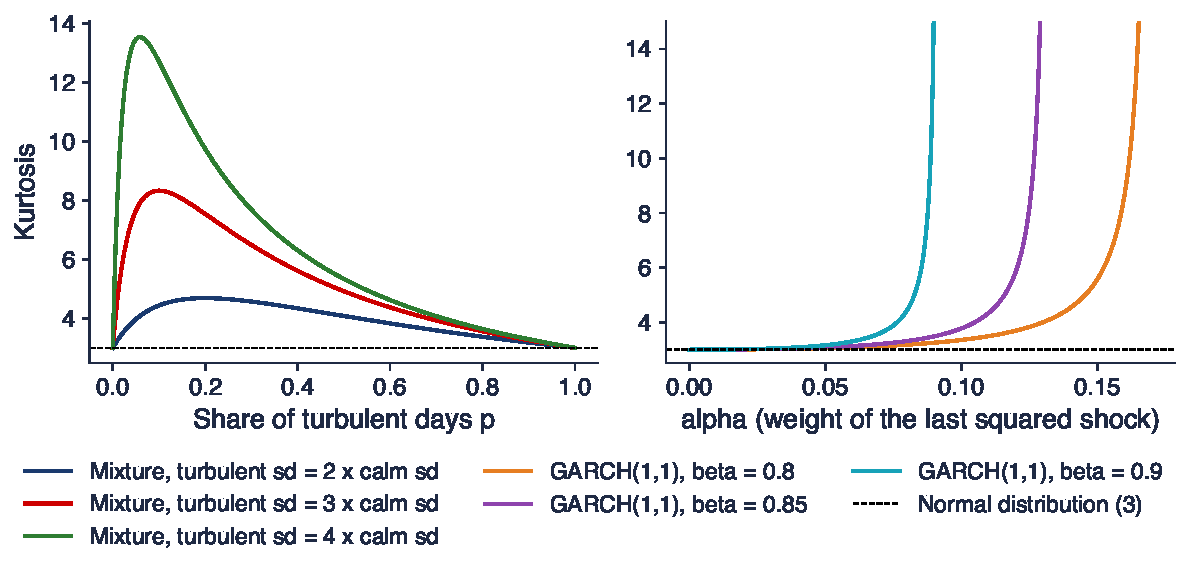
\includegraphics[width=0.97\textwidth,height=0.56\textheight,keepaspectratio]{sfm_ch8_kurtosis.pdf}
\end{center}
\vspace{-0.25cm}
\begin{itemize}
    \item Stînga: zile liniștite cu abaterea standard 1, zile agitate cu abaterea standard 2 (ponderea $p = 0{,}2$): $E[\sigma^2] = 1{,}6$, $E[\sigma^4] = 4{,}0$, coeficientul de boltire $3E[\sigma^4]/E[\sigma^2]^2 = 4{,}69$, deși fiecare zi este Normală
    \item Dreapta: coeficientul de boltire al unui GARCH(1,1), $3 + 6\alpha^2/(1 - \beta^2 - 2\alpha\beta - 3\alpha^2)$, ca în SFEkurgarch; $\alpha = 0{,}10$, $\beta = 0{,}85$: 3{,}77 (\sfmchlink{https://danpele.github.io/SFM/RO/Cursuri/capitol9_modele_arch_garch.pdf}{Capitolul 9})
\end{itemize}
\sfmquantlet{Ch_08}{SFM_ch8_kurgarch}
\end{frame}

\begin{frame}{Recapitulare: volatility clustering}
\itemsize{\small}
\begin{itemize}
    \item $r_t$ aproape necorelat, $|r_t|$ și $r_t^2$ corelate puternic și persistent: volatility clustering
    \item Testele: Ljung--Box pe $r_t^2$ (McLeod--Li) și ARCH-LM $= nR^2$; ambele resping pe toate piețele
    \item Volatility clustering ține de ordinea randamentelor și este una dintre sursele cozilor groase
\end{itemize}
\end{frame}


%=============================================================================
\section{Comportamentul pe termen lung, VIX și efectul de levier}
%=============================================================================

\begin{frame}{Volatilitatea în trei decenii}
\itemsize{\footnotesize}
\begin{center}
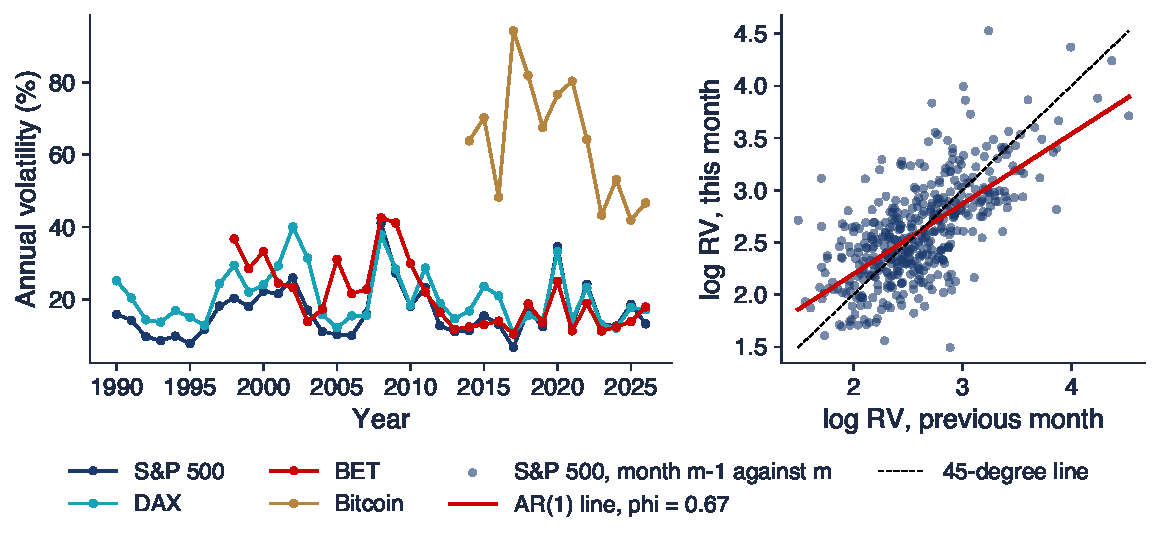
\includegraphics[width=0.97\textwidth,height=0.50\textheight,keepaspectratio]{sfm_ch8_long_term.pdf}
\end{center}
\vspace{-0.25cm}
\begin{itemize}
    \item Stînga: volatilitatea fiecărui an calendaristic (anualizată, \%); dreapta: logaritmul volatilității realizate lunare a S\&P 500 (din randamente zilnice) față de luna precedentă
    \item S\&P 500: de la 7\% (2017) la 41\% (2008); BET: de la 10\% (2017) la 43\% (2008); Bitcoin: de la 42\% (2025) la 94\% (2017)
\end{itemize}
\sfmquantlet{Ch_08}{SFM_ch8_long_term_vix}
\end{frame}

\begin{frame}{Interpretarea persistenței și a revenirii la medie}
\itemsize{\small}
\begin{itemize}
    \item Volatilitatea se schimbă în timp, dar nu se îndepărtează la nesfîrșit: revine la un nivel normal \refSchwert
    \begin{itemize}
        \item AR(1) pentru logaritmul volatilității realizate lunare a S\&P 500 (441 de luni): $\hat\phi = 0{,}67$ (SE 0{,}04)
        \item timpul de înjumătățire al unui șoc de volatilitate: $\ln 0{,}5/\ln\hat\phi = 1{,}7$ luni; nivelul de lungă durată circa 13{,}5\%
    \end{itemize}
    \item Volatilitatea lunară are asimetrie la dreapta (coeficientul de asimetrie 3{,}3), logaritmul ei mult mai puțin (0{,}6) \refABDE
    \begin{itemize}
        \item media 15{,}3\% este peste mediana 12{,}9\%: cîteva luni de criză trag media în sus
        \item de aceea modelele volatilității sînt adesea scrise pentru $\ln\sigma_t$
    \end{itemize}
    \item Revenirea la medie este exact ce îi lipsește modelului EWMA și ce are GARCH cu $\alpha + \beta < 1$ (\sfmchlink{https://danpele.github.io/SFM/RO/Cursuri/capitol9_modele_arch_garch.pdf}{Capitolul 9})
\end{itemize}\sfmquantlet{Ch_08}{SFM_ch8_long_term_vix}
\end{frame}

\begin{frame}{VIX: volatilitatea implicită}
\itemsize{\small}
\begin{columns}[T]
\begin{column}{0.58\textwidth}
\begin{itemize}
    \item Opțiunile se tranzacționează la bursă din 1973, cînd membrii bursei Chicago Board of Trade au înființat \textbf{CBOE} (Chicago Board Options Exchange)
    \begin{itemize}
        \item prețul unei opțiuni depinde de volatilitatea pe care piața o așteaptă pînă la scadență
        \item \textbf{volatilitatea implicită}: volatilitatea care, introdusă într-o formulă de evaluare a opțiunilor, dă prețul observat
    \end{itemize}
    \item \textbf{VIX}, introdus în 1993 \refWhaley: volatilitatea așteptată a S\&P 500 pentru următoarele 30 de zile calendaristice, din prețurile opțiunilor pe S\&P 500 \refCboe
    \begin{itemize}
        \item exprimat în procente anualizate: VIX $= 20$ înseamnă circa $20/\sqrt{12} \approx 5{,}8\%$ pe o lună
        \item numit „indicele fricii”: crește brusc cînd acțiunile scad \refWhaleyB
    \end{itemize}
\end{itemize}
\end{column}
\begin{column}{0.38\textwidth}
\centering
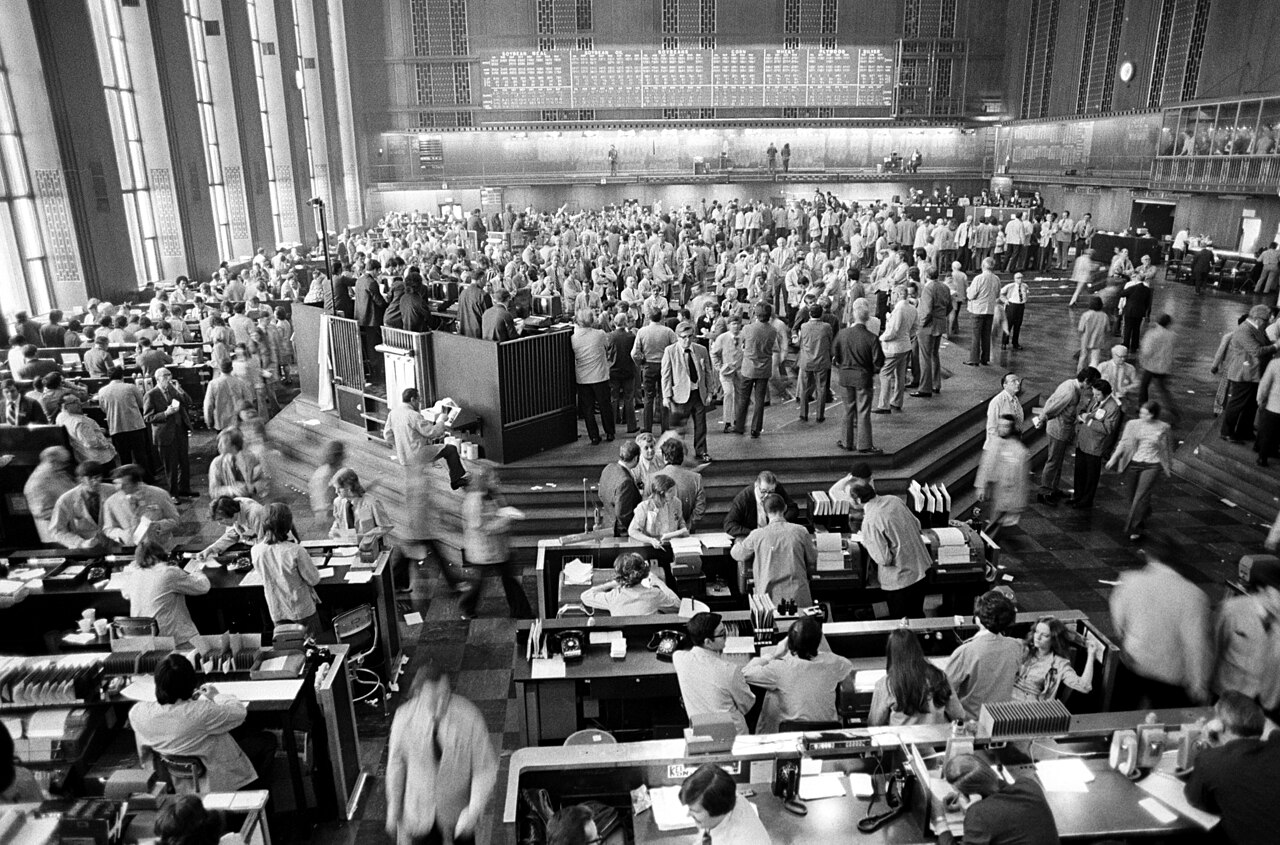
\includegraphics[height=0.34\textheight]{ch8_cbot_1973.jpg}\\[1mm]
\imgcap{Agenți de bursă la Chicago Board of Trade, 31 mai 1973}
\imgcredit{https://commons.wikimedia.org/wiki/File:20120105-OC-AMW-0425_(7042322619).jpg}{Foto: U.S. Department of Agriculture (1973); domeniu public; Wikimedia Commons}
\end{column}
\end{columns}
\end{frame}

\begin{frame}{VIX față de volatilitatea care a urmat}
\itemsize{\footnotesize}
\begin{center}
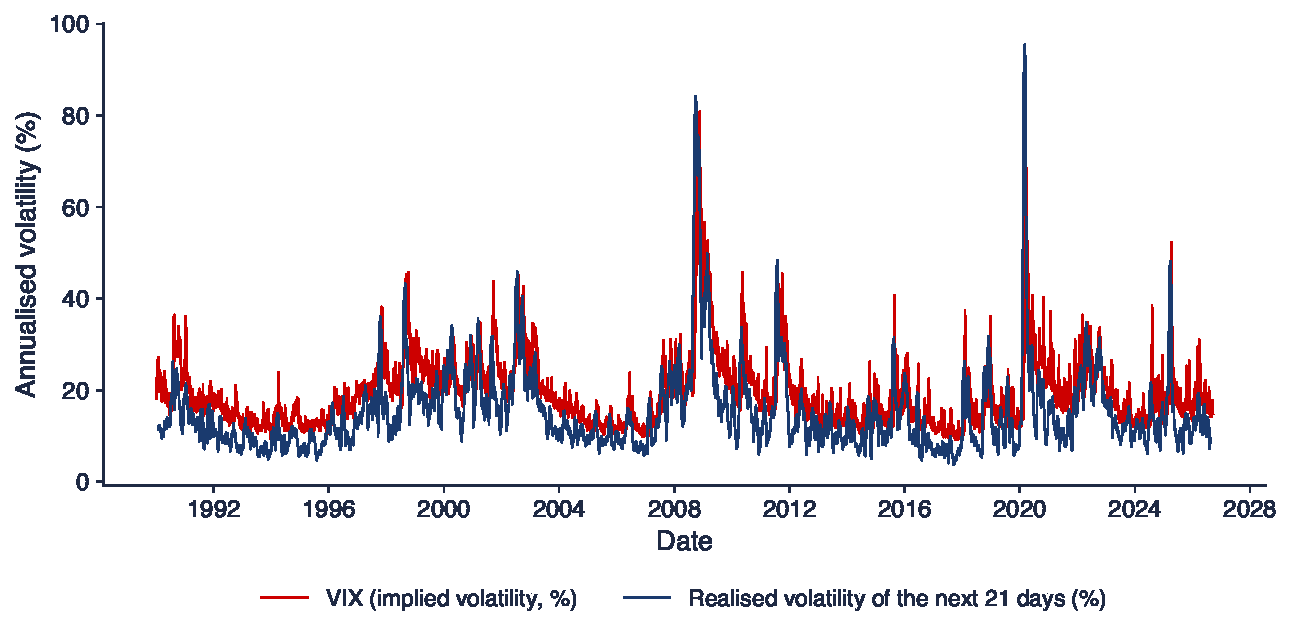
\includegraphics[width=0.97\textwidth,height=0.52\textheight,keepaspectratio]{sfm_ch8_vix.pdf}
\end{center}
\vspace{-0.25cm}
\begin{itemize}
    \item VIX și volatilitatea realizată a S\&P 500 în următoarele 21 de zile de tranzacționare, $\sqrt{(a/21)\sum_{j=1}^{21} r_{t+j}^2}$; maximul VIX: 82{,}7 pe 16 martie 2020
    \item \textbf{Întrebare pentru sală}: linia roșie este de obicei deasupra sau sub cea albastră?
\end{itemize}
\sfmquantlet{Ch_08}{SFM_ch8_long_term_vix}
\end{frame}

\begin{frame}{Interpretarea relației dintre volatilitatea implicită și cea realizată}
\itemsize{\small}
\begin{itemize}
    \item \textbf{Răspuns}: deasupra; VIX a depășit volatilitatea realizată din următoarele 21 de zile în 86\% din cele 9\,199 de zile
    \begin{itemize}
        \item media VIX 19{,}4\% față de media volatilității realizate 15{,}3\%: o diferență de 4{,}1 puncte
        \item \textbf{prima de risc a varianței}: investitorii plătesc pentru a fi asigurați împotriva salturilor de volatilitate \refCW, \refBTZ
    \end{itemize}
    \item Ca prognoză, VIX este informativ, dar deplasat
    \begin{itemize}
        \item regresia volatilității realizate viitoare pe VIX: realizată $= -1{,}72 + 0{,}88\,$VIX, $R^2 = 0{,}52$
        \item volatilitatea realizată din ultimele 21 de zile explică mai puțin: $R^2 = 0{,}44$
    \end{itemize}
    \item Variațiile zilnice ale logaritmului VIX și randamentele S\&P 500: corelație $-0{,}71$: frica crește cînd prețurile scad
\end{itemize}\sfmquantlet{Ch_08}{SFM_ch8_long_term_vix}
\end{frame}

\begin{frame}{Efectul de levier}
\itemsize{\small}
\begin{itemize}
    \item \textbf{Efectul de levier}: randamentele negative sînt urmate de o volatilitate mai mare decît randamentele pozitive de aceeași mărime \refChristie
    \begin{itemize}
        \item explicația prin levier: scăderea prețului acțiunii crește raportul datorii/capital propriu, deci acțiunea devine mai riscantă
        \item explicația prin feedback de volatilitate: o volatilitate așteptată mai mare crește randamentul cerut, deci prețul scade azi \refFSS, \refBW
    \end{itemize}
    \item O măsură simplă: $\mathrm{corr}(r_t, |r_{t+j}|)$ pentru $j = 1, 2, \dots$
    \begin{itemize}
        \item negativă: căderea de azi anunță agitația de mîine; zero într-un model simetric
    \end{itemize}
    \item \sfmchlink{https://danpele.github.io/SFM/RO/Cursuri/capitol2_distributii_clasice_fapte_stilizate.pdf}{Capitolul 2} a arătat asimetria distribuției; aici asimetria apare în \textbf{dinamica} volatilității
\end{itemize}
\end{frame}

\begin{frame}{Veștile proaste cresc volatilitatea viitoare}
\itemsize{\footnotesize}
\begin{center}
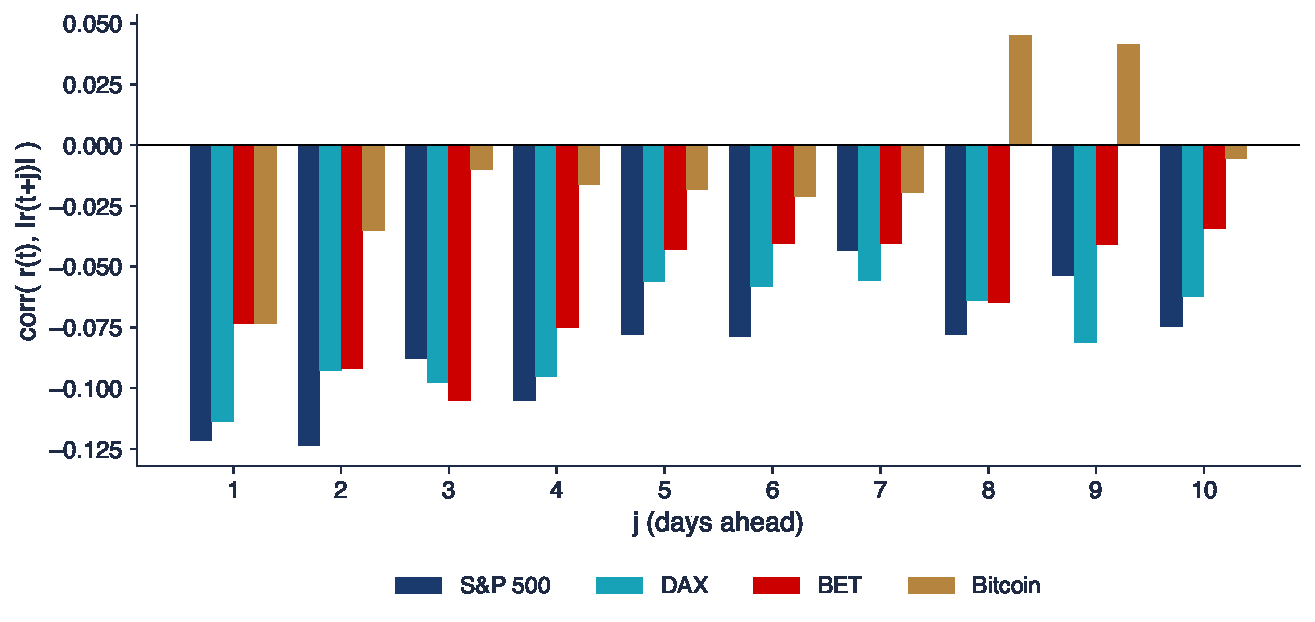
\includegraphics[width=0.97\textwidth,height=0.52\textheight,keepaspectratio]{sfm_ch8_leverage.pdf}
\end{center}
\vspace{-0.25cm}
\begin{itemize}
    \item $\mathrm{corr}(r_t, |r_{t+j}|)$, $j = 1, \dots, 10$; S\&P 500: $-0{,}122$ la $j = 1$; în sens invers, $\mathrm{corr}(|r_{t-1}|, r_t) = 0{,}025$
    \item Media lui $r_{t+1}^2$ după o zi de scădere împărțită la cea după o zi de creștere: S\&P 500 1{,}51, DAX 1{,}46, BET 1{,}41, Bitcoin 1{,}06
\end{itemize}
\sfmquantlet{Ch_08}{SFM_ch8_leverage}
\end{frame}

\begin{frame}{Volatilitatea neparametrică în funcție de randamentul de ieri}
\itemsize{\footnotesize}
\begin{center}
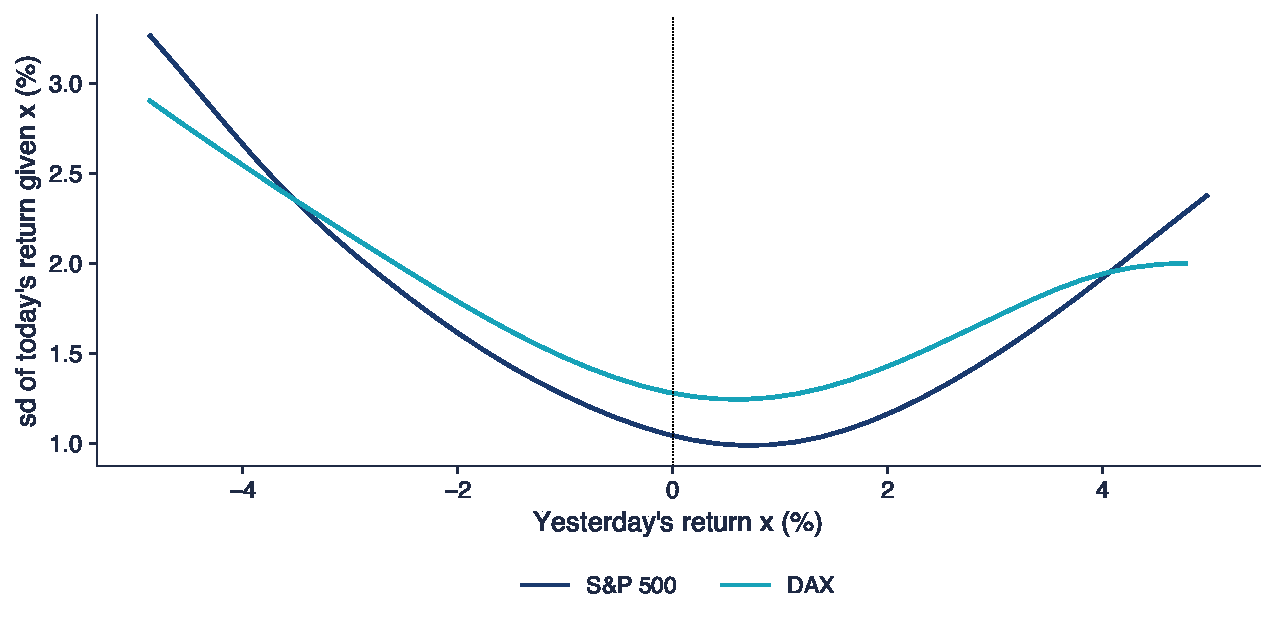
\includegraphics[width=0.97\textwidth,height=0.48\textheight,keepaspectratio]{sfm_ch8_news_impact.pdf}
\end{center}
\vspace{-0.25cm}
\begin{itemize}
    \item $\hat\sigma(x) = \sqrt{\hat m_2(x) - \hat m_1(x)^2}$, $\hat m_1$, $\hat m_2$: regresii liniare locale ale lui $r_t$ și $r_t^2$ pe $r_{t-1} = x$ (nucleu cvartic, lățimea de bandă $0{,}04$ pe randamente zecimale, ca în SFEvolnonparest)
    \item S\&P 500: $\hat\sigma(-2\%) = 1{,}61\%$ față de $\hat\sigma(+2\%) = 1{,}16\%$; minimul este la $x \approx 0{,}7\%$, nu la 0: un impact asimetric al știrilor
\end{itemize}
\sfmquantlet{Ch_08}{SFM_ch8_leverage}
\end{frame}

\begin{frame}{Recapitulare: comportamentul pe termen lung, VIX și efectul de levier}
\itemsize{\small}
\begin{itemize}
    \item Volatilitatea este persistentă, dar revine la medie: timp de înjumătățire de circa 1{,}7 luni la S\&P 500
    \item VIX (volatilitatea implicită) este peste volatilitatea realizată în 86\% din zile: o primă de risc a varianței
    \item Efectul de levier: scăderile cresc volatilitatea viitoare la indicii bursieri; mai slab și de mai scurtă durată la Bitcoin
\end{itemize}
\end{frame}


%=============================================================================
\section{Evaluarea prognozelor de volatilitate}
%=============================================================================

\begin{frame}{Problema variabilei proxy}
\itemsize{\small}
\begin{itemize}
    \item O prognoză $h_t$ a lui $\sigma_t^2$ se face la închiderea zilei $t-1$; valoarea reală $\sigma_t^2$ nu este observată niciodată
    \begin{itemize}
        \item comparăm $h_t$ cu o variabilă \textbf{proxy} $\hat\sigma_t^2$: o mărime măsurabilă cu $E[\hat\sigma_t^2 \mid \mathcal{F}_{t-1}] = \sigma_t^2$
    \end{itemize}
    \item Variabile proxy, de la zgomotoase la precise: $r_t^2$, un estimator de amplitudine, varianța realizată
    \begin{itemize}
        \item cu $r_t^2$ chiar și o prognoză perfectă pare slabă: \refAB{} au arătat că un $R^2$ mic nu înseamnă un model prost
    \end{itemize}
    \item \textbf{Regresia Mincer--Zarnowitz} \refMZ: $\hat\sigma_t^2 = a + b\,h_t + u_t$
    \begin{itemize}
        \item o prognoză bună are $a \approx 0$, $b \approx 1$; $R^2$ măsoară ce parte din variația variabilei proxy este explicată de prognoză
    \end{itemize}
\end{itemize}
\end{frame}

\begin{frame}{Funcții de pierdere: MSE și QLIKE}
\itemsize{\small}
\begin{itemize}
    \item Pierderea medie pe zilele de evaluare; o valoare mai mică este mai bună \refPatton
    \begin{itemize}
        \item MSE: $L = (\hat\sigma_t^2 - h_t)^2$
        \item \textbf{QLIKE} (quasi-likelihood, cvasi-verosimilitate): $L = \hat\sigma_t^2/h_t + \ln h_t$, adică, pînă la constante, opusul log-verosimilității Normale
    \end{itemize}
    \item Ambele sînt \textbf{robuste}: cu o variabilă proxy zgomotoasă, dar nedeplasată, ordonează prognozele la fel ca varianța reală
    \begin{itemize}
        \item pierderile calculate pe $\sqrt{h_t}$ sau pe $\ln h_t$ nu sînt robuste și pot prefera prognoza greșită
    \end{itemize}
    \item \textbf{Exemplu rezolvat}: varianța reală și variabila proxy egale cu 1; două prognoze, $h = 0{,}5$ și $h = 2$
    \begin{itemize}
        \item MSE: $(1 - 0{,}5)^2 = 0{,}25$ față de $(1 - 2)^2 = 1$: MSE penalizează mai mult supraestimarea
        \item QLIKE: $1/0{,}5 + (-0{,}693) = 1{,}307$ față de $1/2 + 0{,}693 = 1{,}193$: QLIKE penalizează mai mult subestimarea, eroarea costisitoare în managementul riscului
    \end{itemize}
\end{itemize}
\end{frame}

\begin{frame}{S\&P 500: care prognoză este cea mai bună?}
\itemsize{\footnotesize}
\begin{center}
\footnotesize
\begin{tabular}{lrrrrrr}
\toprule
& \textbf{21 de zile} & \textbf{63 de zile} & \textbf{252 de zile} & \textbf{EWMA 0,94} & \textbf{EWMA 0,97} & \textbf{VIX} \\
\midrule
MSE & 18{,}99 & 20{,}77 & 21{,}43 & 17{,}77 & 19{,}02 & 16{,}70 \\
QLIKE & 0{,}876 & 0{,}914 & 1{,}099 & 0{,}808 & 0{,}844 & 0{,}799 \\
MZ $R^2$, proxy $r^2$ & 0{,}14 & 0{,}05 & 0{,}01 & 0{,}17 & 0{,}11 & 0{,}25 \\
MZ $R^2$, proxy de amplitudine & 0{,}24 & 0{,}09 & 0{,}02 & 0{,}29 & 0{,}19 & 0{,}42 \\
\bottomrule
\end{tabular}
\end{center}
\begin{itemize}
    \item Prognoze ale varianței pentru ziua următoare, pentru 4\,202 de zile, începînd din 2010; proxy $r_t^2$; prognoza VIX: VIX$^2/a$; proxy de amplitudine: $o_t^2$ plus termenul Garman--Klass
    \item Testul \textbf{DM} (Diebold--Mariano) al egalității QLIKE \refDM: EWMA 0,94 față de 21 de zile $t = -4{,}50$ (p $<$\,0{,}001); VIX față de EWMA 0,94 $t = -0{,}32$ (p = 0{,}751)
    \item EWMA este semnificativ mai bun decît fereastra de 21 de zile; VIX și EWMA nu diferă semnificativ; fereastra lungă este cea mai slabă; o variabilă proxy precisă crește fiecare $R^2$, dar nu schimbă ordinea
\end{itemize}\sfmquantlet{Ch_08}{SFM_ch8_forecast_evaluation}
\end{frame}

\begin{frame}{Prognozele din 2020}
\itemsize{\footnotesize}
\begin{center}
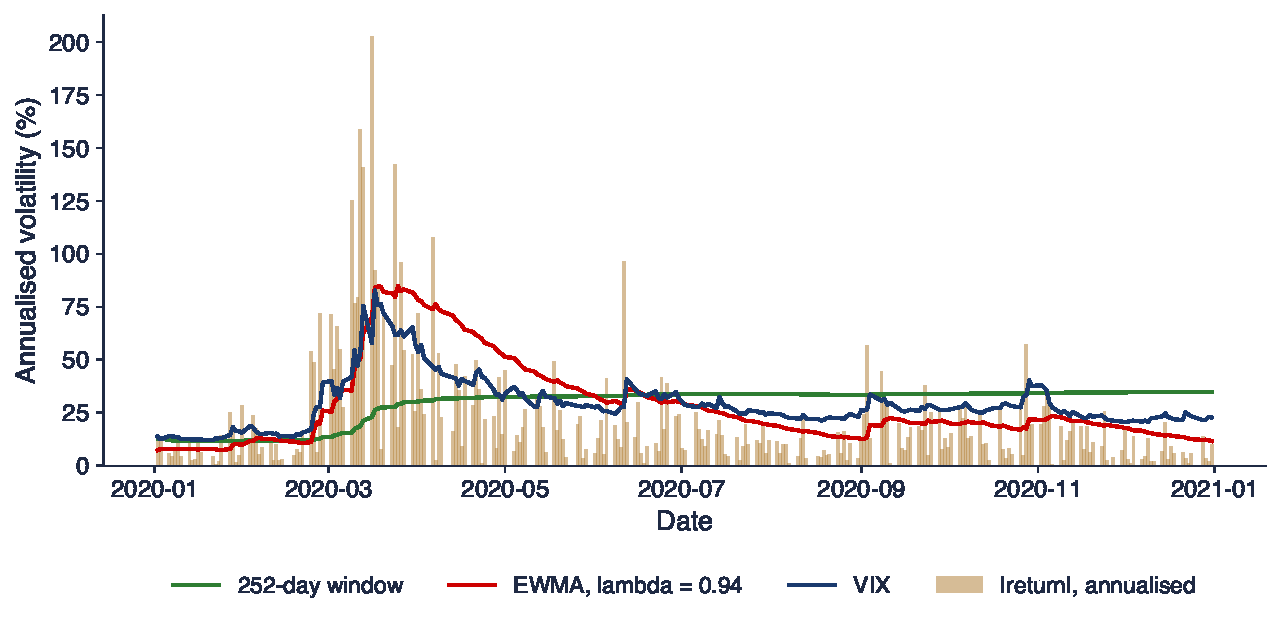
\includegraphics[width=0.97\textwidth,height=0.52\textheight,keepaspectratio]{sfm_ch8_forecast_paths.pdf}
\end{center}
\vspace{-0.25cm}
\begin{itemize}
    \item Prognozele volatilității S\&P 500 pentru ziua următoare în 2020 (anualizate): fereastra de 252 de zile, EWMA ($\lambda = 0{,}94$) și VIX; barele: $|r_t|$
    \item VIX a început să crească cu o zi de tranzacționare înaintea primei scăderi mari din februarie 2020; EWMA a crescut imediat după ea; fereastra de 252 de zile s-a mișcat lent și a rămas aproape de vîrf pînă la sfîrșitul anului
\end{itemize}
\sfmquantlet{Ch_08}{SFM_ch8_forecast_evaluation}
\end{frame}

\begin{frame}{Alegerea lui $\lambda$ după QLIKE}
\itemsize{\footnotesize}
\begin{center}
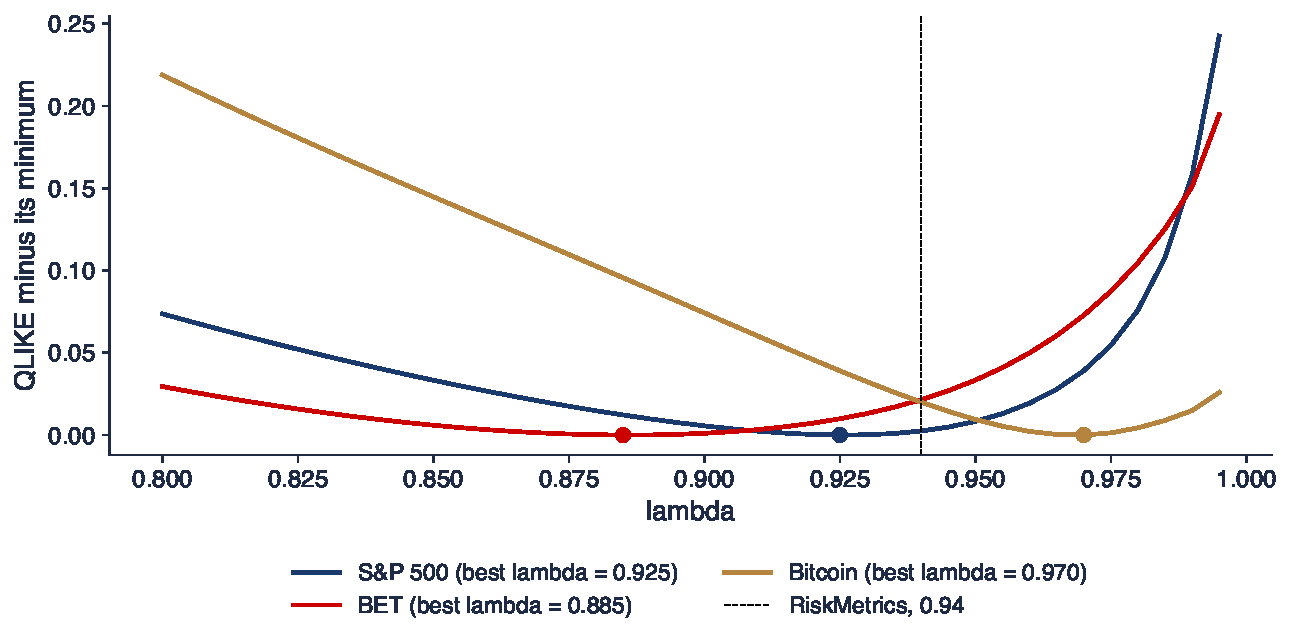
\includegraphics[width=0.97\textwidth,height=0.48\textheight,keepaspectratio]{sfm_ch8_lambda.pdf}
\end{center}
\vspace{-0.25cm}
\begin{itemize}
    \item QLIKE mediu al prognozelor EWMA pentru ziua următoare (proxy $r_t^2$, din 2010; Bitcoin din 2016) minus minimul lui, pentru $\lambda$ între 0,80 și 0,995
    \item Cel mai bun $\lambda$: S\&P 500 0{,}925, BET 0{,}885, Bitcoin 0{,}970; valoarea RiskMetrics 0,94 pierde doar 0{,}002 la S\&P 500
    \item Un singur $\lambda$ pentru toate activele este un compromis comod, nu un optim
\end{itemize}
\sfmquantlet{Ch_08}{SFM_ch8_forecast_evaluation}
\end{frame}

\begin{frame}{Recapitulare: evaluarea prognozelor de volatilitate}
\itemsize{\small}
\begin{itemize}
    \item Comparăm prognozele cu o variabilă proxy; $r_t^2$ este nedeplasat, dar zgomotos, deci valorile $R^2$ sînt mici chiar și pentru prognoze bune
    \item Folosiți pierderi robuste (MSE, QLIKE) și testați diferențele (Diebold--Mariano); o comparație amplă a modelelor de volatilitate: \refHL
    \item S\&P 500: EWMA și VIX sînt cele mai bune prognoze simple; ferestrele lungi sînt cele mai slabe
\end{itemize}
\end{frame}


%=============================================================================
\section{AI pentru descoperire științifică}
%=============================================================================

\begin{frame}{O întrebare deschisă}
\itemsize{\small}
\begin{itemize}
    \item \textbf{Ajută estimatorii de amplitudine la Bursa de Valori București, unde multe acțiuni se tranzacționează rar?}
    \begin{itemize}
        \item teoria: amplitudinile sînt de 5--9 ori mai eficiente; dar tranzacționarea rară micșorează amplitudinea observată (secțiunea 4)
        \item zile cu tranzacții, dar cu închiderea neschimbată, din 2010: TLV 9\%, SNP 8\%, BRD 10\%, TGN 10\%
        \item raportul volatilităților Parkinson / închidere--închidere: TLV 0{,}81, SNP 0{,}87, BRD 0{,}90, TGN 0{,}87 (S\&P 500: 0{,}78)
        \item QLIKE al prognozelor pentru ziua următoare, cu fereastra de 21 de zile, CC față de YZ: TLV 2{,}022 față de 2{,}039; TGN 1{,}750 față de 1{,}636
    \end{itemize}
    \item Întrebarea rămîne deschisă: răspunsul diferă de la o acțiune la alta; contează lichiditatea, licitația de deschidere sau mărimea mișcării overnight?
    \item Instrumentele AI pot accelera un astfel de studiu; nu înlocuiesc verificarea lui \refWang
\end{itemize}\sfmquantlet{Ch_08}{SFM_ch8_bvb_range}
\end{frame}

\begin{frame}{Contribuția posibilă a AI}
\itemsize{\small}
\begin{itemize}
    \item \textbf{Literatura}: o listă a studiilor despre volatilitatea de amplitudine și cea realizată pe piețe emergente și puțin lichide, cu datele și estimatorii folosiți
    \item \textbf{Cod}: o primă versiune a celor cinci estimatori, a prognozelor pe ferestre mobile și a comparațiilor QLIKE pentru toate acțiunile din BET
    \item \textbf{Robustețe}: grupe de lichiditate după volum, alte ferestre, cele două jumătăți 2016--2020 și 2021--2026
    \item Exemplu de prompt
    \begin{itemize}
        \item \aiprompt{Write a Python function that computes the Parkinson, Garman-Klass, Rogers-Satchell and Yang-Zhang variance on rolling 21-day windows from daily open, high, low and close prices, and compares their next-day forecasts with QLIKE against squared close-to-close returns.}
    \end{itemize}
\end{itemize}
\end{frame}

\begin{frame}{Verificări necesare}
\itemsize{\small}
\begin{itemize}
    \item Constantele: $4\ln 2$ la Parkinson, $2\ln 2 - 1$ la Garman--Klass, $k$ la Yang--Zhang; o ciornă cu $\ln 2$ sau cu $k = 0{,}34$ este greșită
    \item Prețurile acțiunilor: deschiderea, maximul și minimul trebuie ajustate pentru dividende și splituri cu același factor ca închiderea
    \item Anualizarea cu frecvența reală: 365 pentru cripto, circa 250 pentru acțiunile BVB
    \item Fără informație din viitor: prognoza pentru ziua $t$ folosește doar datele pînă în ziua $t-1$
    \item Referințele: fiecare lucrare citată trebuie să existe; verificați DOI-ul
\end{itemize}
\end{frame}

\begin{frame}{Idee de proiect}
\itemsize{\small}
\begin{itemize}
    \item \textbf{Întrebarea}: ce estimator zilnic de volatilitate ar trebui să folosească un manager de risc din România?
    \begin{itemize}
        \item date: acțiuni BVB din 2010 (TLV, SNP, BRD, TGN și altele cu date OHLC), S\&P 500 și DAX ca termeni de comparație (EODHD)
    \end{itemize}
    \item Pași
    \begin{itemize}
        \item cei cinci estimatori pe ferestre de 21 de zile; variantele EWMA ale fiecăruia; prognoze pentru ziua următoare
        \item QLIKE și MSE cu proxy-ul $r_t^2$; teste Diebold--Mariano; rezultate pe grupe de lichiditate
        \item legați cîștigul YZ față de CC de ponderea zilelor fără volum și de ponderea nopții
    \end{itemize}
    \item Livrabile: un tabel, un grafic și un paragraf despre ce pot și ce nu pot arăta datele
    \item Declarați orice utilizare a instrumentelor AI și enumerați erorile acestora pe care le-ați corectat
\end{itemize}
\end{frame}


%=============================================================================
\section{Rezumat}
%=============================================================================

\begin{frame}{Idei de reținut}
\itemsize{\small}
\begin{itemize}
    \item Volatilitatea este abaterea standard a randamentelor; este latentă și variază în timp; se anualizează cu frecvența reală
    \item La ferestrele istorice, viteza de reacție se plătește cu zgomot; EWMA ($\lambda = 0{,}94$) reacționează repede și evită ghost effect
    \item Estimatorii de amplitudine folosesc traiectoria zilei: mult mai eficienți, dar deplasați de salturile overnight și de tranzacționarea rară; Yang--Zhang adaugă noaptea
    \item Volatility clustering: $|r_t|$ și $r_t^2$ sînt autocorelate; se detectează cu Ljung--Box pe $r_t^2$ și cu ARCH-LM
    \item Volatilitatea revine la medie; VIX depășește de obicei volatilitatea realizată; scăderile cresc volatilitatea viitoare
    \item Comparați prognozele cu pierderi robuste (QLIKE) și o variabilă proxy; testați diferențele
\end{itemize}
\end{frame}

\begin{frame}{Formule de reținut}
\itemsize{\small}
{\renewcommand{\arraystretch}{1.4}\begin{center}
\scriptsize
\begin{tabular}{ll}
\toprule
\textbf{Mărimea} & \textbf{Formula} \\
\midrule
Volatilitatea anualizată & $\sigma_{\text{an}} = \sigma_{\text{zi}}\sqrt{a}$ \\
EWMA & $\sigma_t^2 = \lambda\sigma_{t-1}^2 + (1-\lambda)r_{t-1}^2$, \quad timp de înjumătățire $\ln 0{,}5/\ln\lambda$ \\
Parkinson & $(u_t - d_t)^2/(4\ln 2)$ \\
Garman--Klass & $0{,}5(u_t - d_t)^2 - (2\ln 2 - 1)c_t^2$ \\
Rogers--Satchell & $u_t(u_t - c_t) + d_t(d_t - c_t)$ \\
Yang--Zhang & $\hat\sigma_O^2 + k\hat\sigma_C^2 + (1-k)\hat\sigma_{RS}^2$, \quad $k = 0{,}34/(1{,}34 + (n+1)/(n-1))$ \\
Varianța realizată & $\mathrm{RV}_t = \sum_i r_{t,i}^2$ \\
McLeod--Li & $Q(m) = T(T+2)\sum_{k=1}^m \hat\rho_k(r^2)^2/(T-k) \sim \chi^2(m)$ \\
ARCH-LM & $\mathrm{LM} = nR^2 \sim \chi^2(q)$ \\
MSE, QLIKE & $(\hat\sigma_t^2 - h_t)^2$, \quad $\hat\sigma_t^2/h_t + \ln h_t$ \\
\bottomrule
\end{tabular}
\end{center}
}
\end{frame}

\begin{frame}{Autoevaluare}
\itemsize{\small}
\begin{itemize}
    \item \textbf{Întrebare}: o acțiune are $H = 102$, $L = 98$ într-o zi; care este volatilitatea zilnică Parkinson?
    \begin{itemize}
        \item \textbf{Răspuns}: $\ln(102/98) = 4{,}00\%$; $\sqrt{4{,}00^2/2{,}77} = 2{,}40\%$
    \end{itemize}
    \item \textbf{Întrebare}: testul Ljung--Box pe randamente nu respinge, iar pe randamentele la pătrat respinge puternic; ce concluzie trageți?
    \begin{itemize}
        \item \textbf{Răspuns}: media este imprevizibilă, varianța este previzibilă: volatility clustering fără autocorelația randamentelor
    \end{itemize}
    \item \textbf{Întrebare}: de ce nu poate EWMA cu $\lambda = 0{,}94$ să anticipeze revenirea volatilității la nivelul normal?
    \begin{itemize}
        \item \textbf{Răspuns}: $\alpha + \beta = 1$ și $\omega = 0$: prognozele lui sînt constante la orice orizont
    \end{itemize}
    \item Urmează: \sfmchlink{https://danpele.github.io/SFM/RO/Cursuri/capitol9_modele_arch_garch.pdf}{Capitolul 9}, modelele ARCH și GARCH
\end{itemize}
\end{frame}


%=============================================================================
\section{Bibliografie}
%=============================================================================

\begin{frame}{Bibliografie (1/3)}
\itemsize{\tiny}
\begin{itemize}
    \item Alizadeh, S., Brandt, M.W., Diebold, F.X. (2002). \href{https://doi.org/10.1111/1540-6261.00454}{Range-based estimation of stochastic volatility models}. \textit{Journal of Finance}, 57(3), 1047--1091.
    \item Andersen, T.G., Bollerslev, T. (1998). \href{https://doi.org/10.2307/2527343}{Answering the skeptics: yes, standard volatility models do provide accurate forecasts}. \textit{International Economic Review}, 39(4), 885--905.
    \item Andersen, T.G., Bollerslev, T., Diebold, F.X., Ebens, H. (2001). \href{https://doi.org/10.1016/S0304-405X(01)00055-1}{The distribution of realized stock return volatility}. \textit{Journal of Financial Economics}, 61(1), 43--76.
    \item Andersen, T.G., Bollerslev, T., Diebold, F.X., Labys, P. (2003). \href{https://doi.org/10.1111/1468-0262.00418}{Modeling and forecasting realized volatility}. \textit{Econometrica}, 71(2), 579--625.
    \item Barndorff-Nielsen, O.E., Shephard, N. (2002). \href{https://doi.org/10.1111/1467-9868.00336}{Econometric analysis of realized volatility and its use in estimating stochastic volatility models}. \textit{Journal of the Royal Statistical Society, Series B}, 64(2), 253--280.
    \item Bekaert, G., Wu, G. (2000). \href{https://doi.org/10.1093/rfs/13.1.1}{Asymmetric volatility and risk in equity markets}. \textit{Review of Financial Studies}, 13(1), 1--42.
    \item Bollerslev, T. (1986). \href{https://doi.org/10.1016/0304-4076(86)90063-1}{Generalized autoregressive conditional heteroskedasticity}. \textit{Journal of Econometrics}, 31(3), 307--327.
    \item Bollerslev, T., Tauchen, G., Zhou, H. (2009). \href{https://doi.org/10.1093/rfs/hhp008}{Expected stock returns and variance risk premia}. \textit{Review of Financial Studies}, 22(11), 4463--4492.
    \item Borak, S., Härdle, W.K., López-Cabrera, B. (2013). \href{https://doi.org/10.1007/978-3-642-33929-5}{\textit{Statistics of Financial Markets: Exercises and Solutions}}, 2nd ed. Springer.
    \item Carr, P., Wu, L. (2009). \href{https://doi.org/10.1093/rfs/hhn038}{Variance risk premiums}. \textit{Review of Financial Studies}, 22(3), 1311--1341.
    \item Cboe Global Markets (2026). \href{https://www.cboe.com/tradable_products/vix/}{Cboe Volatility Index (VIX)}. Product page and methodology.
    \item Christie, A.A. (1982). \href{https://doi.org/10.1016/0304-405X(82)90018-6}{The stochastic behavior of common stock variances: value, leverage and interest rate effects}. \textit{Journal of Financial Economics}, 10(4), 407--432.
    \item Cont, R. (2001). \href{https://doi.org/10.1080/713665670}{Empirical properties of asset returns: stylized facts and statistical issues}. \textit{Quantitative Finance}, 1(2), 223--236.
    \item Corsi, F. (2009). \href{https://doi.org/10.1093/jjfinec/nbp001}{A simple approximate long-memory model of realized volatility}. \textit{Journal of Financial Econometrics}, 7(2), 174--196.
    \item Diebold, F.X., Mariano, R.S. (1995). \href{https://doi.org/10.1080/07350015.1995.10524599}{Comparing predictive accuracy}. \textit{Journal of Business \& Economic Statistics}, 13(3), 253--263.
    \item Ding, Z., Granger, C.W.J., Engle, R.F. (1993). \href{https://doi.org/10.1016/0927-5398(93)90006-D}{A long memory property of stock market returns and a new model}. \textit{Journal of Empirical Finance}, 1(1), 83--106.
\end{itemize}
\end{frame}

\begin{frame}{Bibliografie (2/3)}
\itemsize{\tiny}
\begin{itemize}
    \item Engle, R.F. (1982). \href{https://doi.org/10.2307/1912773}{Autoregressive conditional heteroscedasticity with estimates of the variance of United Kingdom inflation}. \textit{Econometrica}, 50(4), 987--1007.
    \item Engle, R.F. (2004). \href{https://doi.org/10.1257/0002828041464597}{Risk and volatility: econometric models and financial practice}. \textit{American Economic Review}, 94(3), 405--420.
    \item Franke, J., Härdle, W.K., Hafner, C.M. (2019). \href{https://doi.org/10.1007/978-3-030-13751-9}{\textit{Statistics of Financial Markets: An Introduction}}, 5th ed. Springer.
    \item French, K.R., Schwert, G.W., Stambaugh, R.F. (1987). \href{https://doi.org/10.1016/0304-405X(87)90026-2}{Expected stock returns and volatility}. \textit{Journal of Financial Economics}, 19(1), 3--29.
    \item Garman, M.B., Klass, M.J. (1980). \href{https://doi.org/10.1086/296072}{On the estimation of security price volatilities from historical data}. \textit{Journal of Business}, 53(1), 67--78.
    \item Hansen, P.R., Lunde, A. (2005). \href{https://doi.org/10.1002/jae.800}{A forecast comparison of volatility models: does anything beat a GARCH(1,1)?} \textit{Journal of Applied Econometrics}, 20(7), 873--889.
    \item J.P. Morgan/Reuters (1996). \href{https://www.msci.com/documents/10199/5915b101-4206-4ba0-aee2-3449d5c7e95a}{\textit{RiskMetrics -- Technical Document}}, 4th ed. New York: Morgan Guaranty Trust Company.
    \item Liu, L.Y., Patton, A.J., Sheppard, K. (2015). \href{https://doi.org/10.1016/j.jeconom.2015.02.008}{Does anything beat 5-minute RV? A comparison of realized measures across multiple asset classes}. \textit{Journal of Econometrics}, 187(1), 293--311.
    \item Ljung, G.M., Box, G.E.P. (1978). \href{https://doi.org/10.1093/biomet/65.2.297}{On a measure of lack of fit in time series models}. \textit{Biometrika}, 65(2), 297--303.
    \item Mandelbrot, B. (1963). \href{https://doi.org/10.1086/294632}{The variation of certain speculative prices}. \textit{Journal of Business}, 36(4), 394--419.
    \item McLeod, A.I., Li, W.K. (1983). \href{https://doi.org/10.1111/j.1467-9892.1983.tb00373.x}{Diagnostic checking ARMA time series models using squared-residual autocorrelations}. \textit{Journal of Time Series Analysis}, 4(4), 269--273.
    \item Mincer, J.A., Zarnowitz, V. (1969). \href{https://www.nber.org/books-and-chapters/economic-forecasts-and-expectations-analysis-forecasting-behavior-and-performance/evaluation-economic-forecasts}{The evaluation of economic forecasts}. In J.A. Mincer (ed.), \textit{Economic Forecasts and Expectations}, 3--46. NBER.
    \item Molnár, P. (2012). \href{https://doi.org/10.1016/j.irfa.2011.06.012}{Properties of range-based volatility estimators}. \textit{International Review of Financial Analysis}, 23, 20--29.
    \item Nobel Prize Outreach (2003). \href{https://www.nobelprize.org/prizes/economic-sciences/2003/summary/}{The Sveriges Riksbank Prize in Economic Sciences in Memory of Alfred Nobel 2003: Robert F. Engle III and Clive W.J. Granger}. nobelprize.org.
    \item Parkinson, M. (1980). \href{https://doi.org/10.1086/296071}{The extreme value method for estimating the variance of the rate of return}. \textit{Journal of Business}, 53(1), 61--65.
    \item Patton, A.J. (2011). \href{https://doi.org/10.1016/j.jeconom.2010.03.034}{Volatility forecast comparison using imperfect volatility proxies}. \textit{Journal of Econometrics}, 160(1), 246--256.
\end{itemize}
\end{frame}

\begin{frame}{Bibliografie (3/3)}
\itemsize{\tiny}
\begin{itemize}
    \item Pele, D.T., Lazar, E., Dufour, A. (2017). \href{https://doi.org/10.3390/e19050226}{Information entropy and measures of market risk}. \textit{Entropy}, 19(5), 226.
    \item Pele, D.T., Mazurencu-Marinescu-Pele, M. (2019). \href{https://doi.org/10.3390/e21020102}{Using high-frequency entropy to forecast Bitcoin's daily Value at Risk}. \textit{Entropy}, 21(2), 102.
    \item Poon, S.-H., Granger, C.W.J. (2003). \href{https://doi.org/10.1257/002205103765762743}{Forecasting volatility in financial markets: a review}. \textit{Journal of Economic Literature}, 41(2), 478--539.
    \item Rogers, L.C.G., Satchell, S.E. (1991). \href{https://doi.org/10.1214/aoap/1177005835}{Estimating variance from high, low and closing prices}. \textit{Annals of Applied Probability}, 1(4), 504--512.
    \item Schwert, G.W. (1989). \href{https://doi.org/10.1111/j.1540-6261.1989.tb02647.x}{Why does stock market volatility change over time?} \textit{Journal of Finance}, 44(5), 1115--1153.
    \item Tsay, R.S. (2010). \href{https://doi.org/10.1002/9780470644560}{\textit{Analysis of Financial Time Series}}, 3rd ed. Wiley.
    \item Wang, H., Fu, T., Du, Y., Gao, W., et al. (2023). \href{https://doi.org/10.1038/s41586-023-06221-2}{Scientific discovery in the age of artificial intelligence}. \textit{Nature}, 620, 47--60.
    \item Whaley, R.E. (1993). \href{https://doi.org/10.3905/jod.1993.407868}{Derivatives on market volatility}. \textit{Journal of Derivatives}, 1(1), 71--84.
    \item Whaley, R.E. (2009). \href{https://doi.org/10.3905/JPM.2009.35.3.098}{Understanding the VIX}. \textit{Journal of Portfolio Management}, 35(3), 98--105.
    \item Yang, D., Zhang, Q. (2000). \href{https://doi.org/10.1086/209650}{Drift-independent volatility estimation based on high, low, open, and close prices}. \textit{Journal of Business}, 73(3), 477--492.
\end{itemize}
\end{frame}

\end{document}
